% !TeX root=../main.tex

\chapter{پاسخ سوالات سری سوم}

% دستور زیر باعث عدم‌نمایش شماره صفحه در اولین صفحهٔ این فصل می‌شود.
%\thispagestyle{empty}
\section*{ پاسخ سوال 1}
\subsection*{سوال یکم}

تابع تبدیل سیستم به صورت زیر داده شده است:
\[
\frac{K_s \,k_e \,k_{\textrm{sp}} \,{\left(A_0 +A_i \right)}}{{\left(s\,\tau +1\right)}\,{\left(s\,{A_0 }^2 +s\,{A_i }^2 +{\left(K_p +C\,s\right)}\,{\left(m_a \,s^2 +d\,s+k_e \right)}\right)}}
\]
برای محاسبه ی معادلات حالت این سیستم، از روش تحقق مینیمال استفاده می شود. لازم به ذکر است که این تبدیل به وسیله ی تابع$ tf2ss$ امکان پذیر نیست، چرا که در محاسبه ی آن مقادیر نمادین مورد استفاده قرار گرفته اند. 
برای محاسبه به روش تحقق مینیمال، ابتدا لازم است صورت و مخرج تابع تبدیل به صورت چند جمله ای مرتب در آید.
بنابراین خواهیم داشت:
\[
C_{\textrm{num}} = K_s \,k_e \,k_{\textrm{sp}} \,{\left(A_0 + A_i \right)}
\]
\[
\tiny
C_{\textrm{den}} = \left(\begin{array}{ccccc} 
	K_p \,k_e  & {A_0 }^2 + {A_i }^2 + C \,k_e + K_p \,d + K_p \,k_e \,\tau & C \,d + K_p \,m_a + \tau \,{\left({A_0 }^2 + {A_i }^2 + C \,k_e + K_p \,d \right)} & C \,m_a + \tau \,{\left(C \,d + K_p \,m_a \right)} & C \,m_a \,\tau 
\end{array}\right)
\]
طبق تعریف تحقق مینیمال ارائه شده برای این تمرین، ماتریس های حالت با تعاریف زیر محاسبه می شوند.

\[
G(s) = \frac{Y(s)}{U(s)} = \frac{\beta}{s^n + \alpha_1 s^{n-1} + \dots + \alpha_{n-1}s + \alpha_n}
\]

\[
\dot{x}(t) = 
\begin{bmatrix}
	0 & 1 & 0 & \dots & 0 \\
	0 & 0 & 1 & \dots & 0 \\
	\vdots & \vdots & \vdots & \ddots & \vdots \\
	0 & 0 & 0 & \dots & 1 \\
	-\alpha_n & -\alpha_{n-1} & -\alpha_{n-2} & \dots & -\alpha_1
\end{bmatrix}
x(t)
+
\begin{bmatrix}
	0 \\
	0 \\
	\vdots \\
	0 \\
	\beta
\end{bmatrix}
u(t)
\]
\[
y(t) = 
\begin{bmatrix}
	1 & 0 & 0 & \dots & 0
\end{bmatrix}
x(t)
\]
که در آن:
\[
\begin{aligned}
	\left\{
	\begin{aligned}
		\alpha_1 &= \frac{\left( \tau (K_p m_a + C d) + C m_a \right)}{\tau C m_a} \\
		\alpha_2 &= \frac{\left( \tau (K_p d + C k_e + A_i^2 + A_0^2) + (K_p m_a + C d) \right)}{\tau C m_a} \\
		\alpha_3 &= \frac{\left( \tau K_p k_e + (K_p d + C k_e + A_i^2 + A_0^2) \right)}{\tau C m_a} \\
		\alpha_4 &= \frac{K_p k_e}{\tau C m_a} \\
		\beta &= \frac{k_{sp} K_s k_e (A_i + A_0)}{\tau C m_a}
	\end{aligned} \right. 
\end{aligned}
\]

با این تعاریف، ماتریس های حالت به دست می آیند.
\[
A = \left(\begin{array}{cccc}
	0 & 1 & 0 & 0\\
	0 & 0 & 1 & 0\\
	0 & 0 & 0 & 1\\
	-\frac{C\,m_a \,\tau }{K_p \,k_e } & -\frac{C\,m_a +\tau \,{\left(C\,d+K_p \,m_a \right)}}{K_p \,k_e } & -\frac{C\,d+K_p \,m_a +\tau \,{\left({A_0 }^2 +{A_i }^2 +C\,k_e +K_p \,d\right)}}{K_p \,k_e } & -\frac{{A_0 }^2 +{A_i }^2 +C\,k_e +K_p \,d+K_p \,k_e \,\tau }{K_p \,k_e }
\end{array}\right)
\]

\[
B = \left(\begin{array}{c}
	0\\
	0\\
	0\\
	\frac{K_s \,k_{\textrm{sp}} \,{\left(A_0 +A_i \right)}}{K_p }
\end{array}\right)
\]

\[
C = \left[1, 0, 0, 0\right]
\]

\[
D = 0
\]
\subsection*{سوال دوم}
برای حل سوال دوم، که کنترل سیستم ذکر شده به روش MPC خطی است، لازم است ابتدا معادلات حالت این سیستم در فضای سیمولینک تعریف شوند. 
\begin{figure}[H]
	\centering
	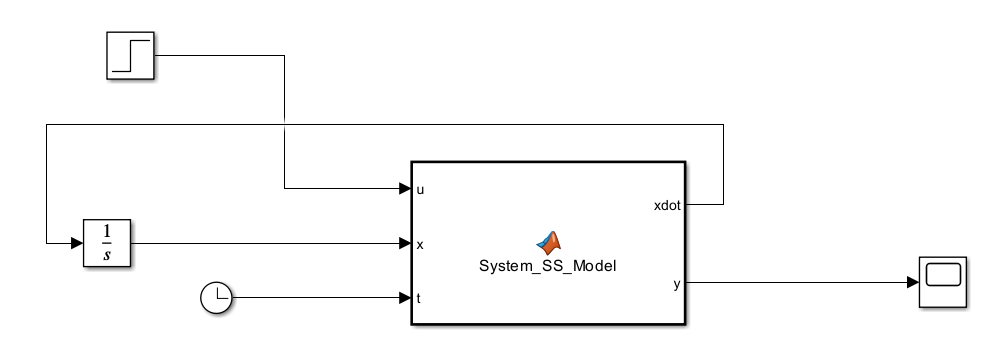
\includegraphics[width=0.7\linewidth]{../img/Q1_OL_diagram}
	\caption{دیاگرام سیستم حلقه باز در محیط سیمولینک}
	\label{fig:q1oldiagram}
\end{figure}
\begin{figure}[H]
	\centering
	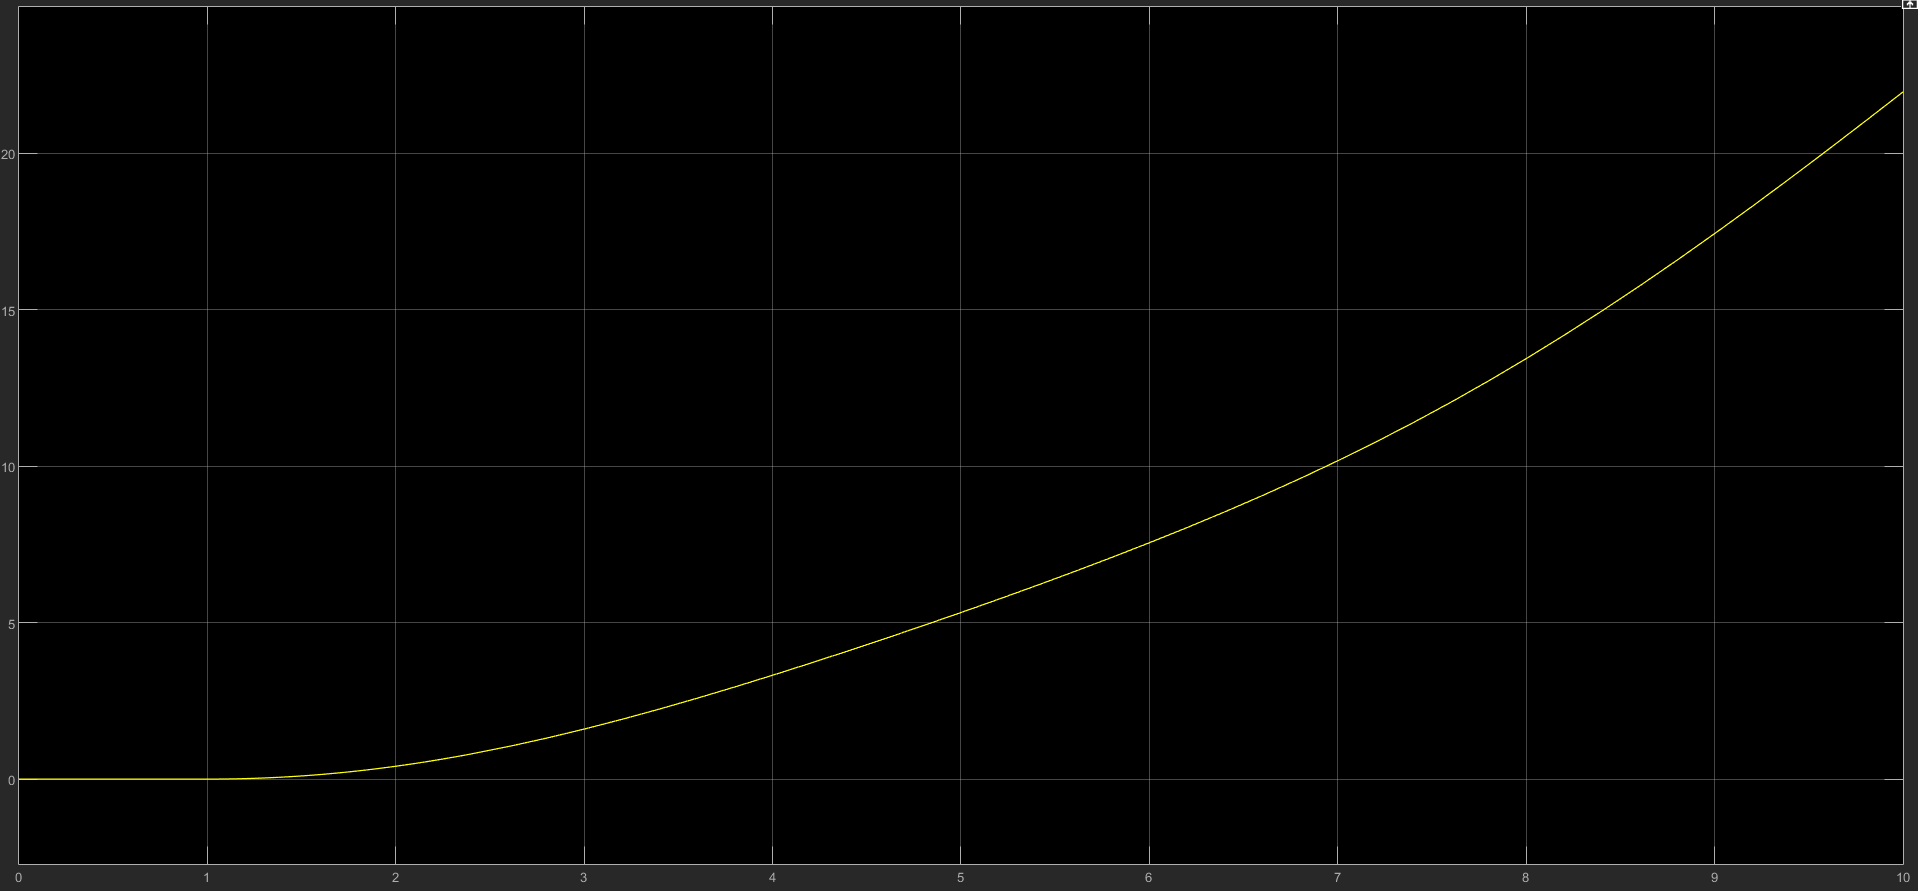
\includegraphics[width=0.7\linewidth]{../img/Q1_OL}
	\caption{پساخ حلقه باز سیستم}
	\label{fig:q1ol}
\end{figure}


همچنین، لحاظ کردن نایقینی های این سیستم در این بخش در نظر گرفته شده است. برای اعمال این نایقینی ها، از تابع سینوسی متغیر با زمان برای اعمال مقادیر انحراف از مقدار واقعی استفاده شده است.
در ادامه، با قرار دادن کنترلر MPC خطی به جای ورودی پله به این سیستم، آن را کنترل خواهیم کرد. برای تنظیم کنترلر پیش بین، از نرخ نمونه برداری 0.01 ثانیه، افق پیش بین 100 و افق کنترلی 20 استفاده شده است.
نمودار تلاش کنترلی و خروجی سیستم در نمودار زیر نمایش داده شده است.
\begin{figure}[H]
	\centering
	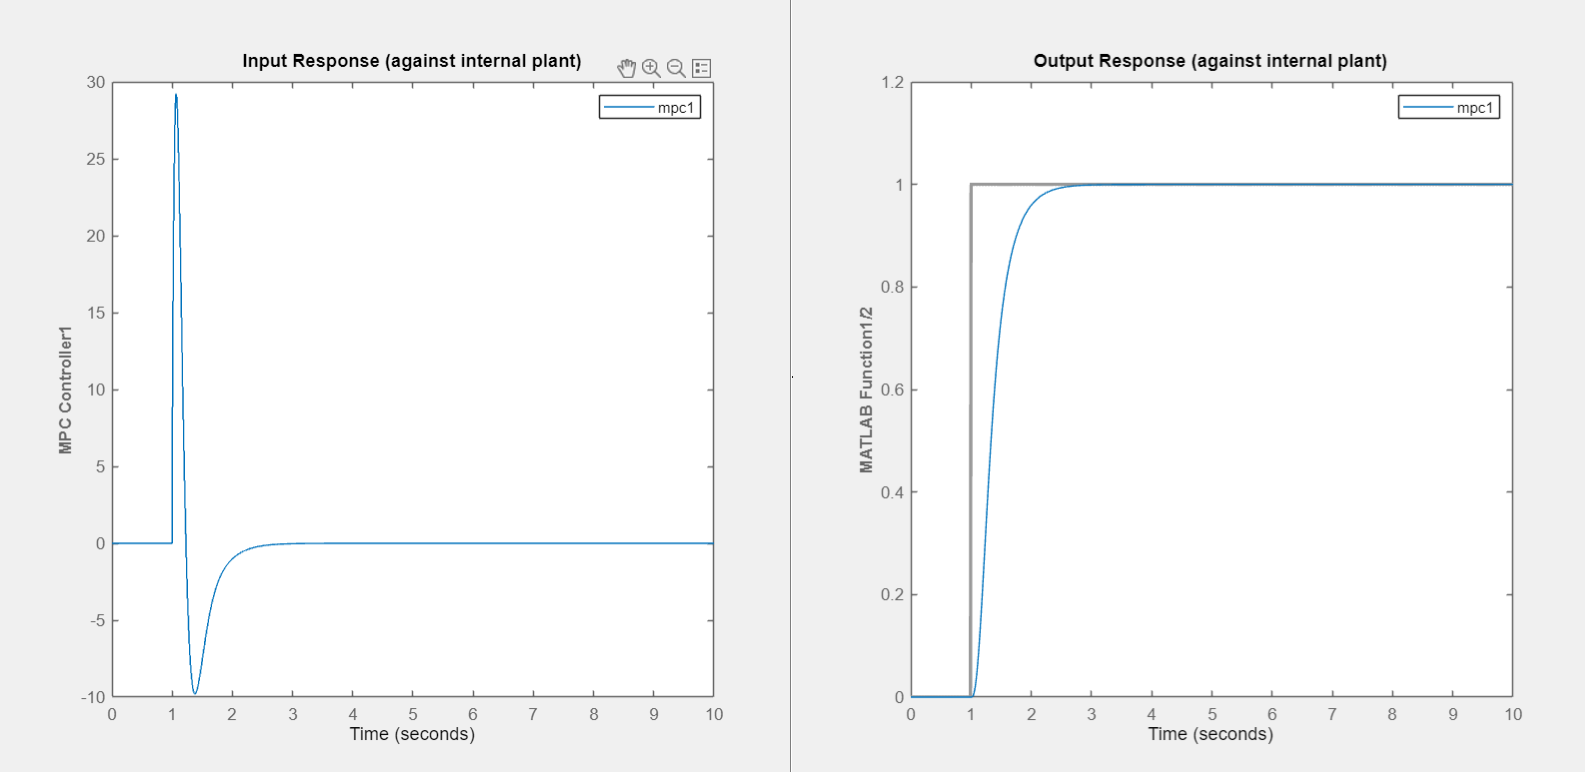
\includegraphics[width=1\linewidth]{../img/Q1_linearMPC_response}
	\caption{تلاش کنترلی و پاسخ سیستم کنترل شده با کنترلر پیش بین خطی}
	\label{fig:q1linearmpcresponse}
\end{figure}
در نتیجه پاسخ سیستم به صورت زیر به دست می آید.
\begin{figure}[H]
	\centering
	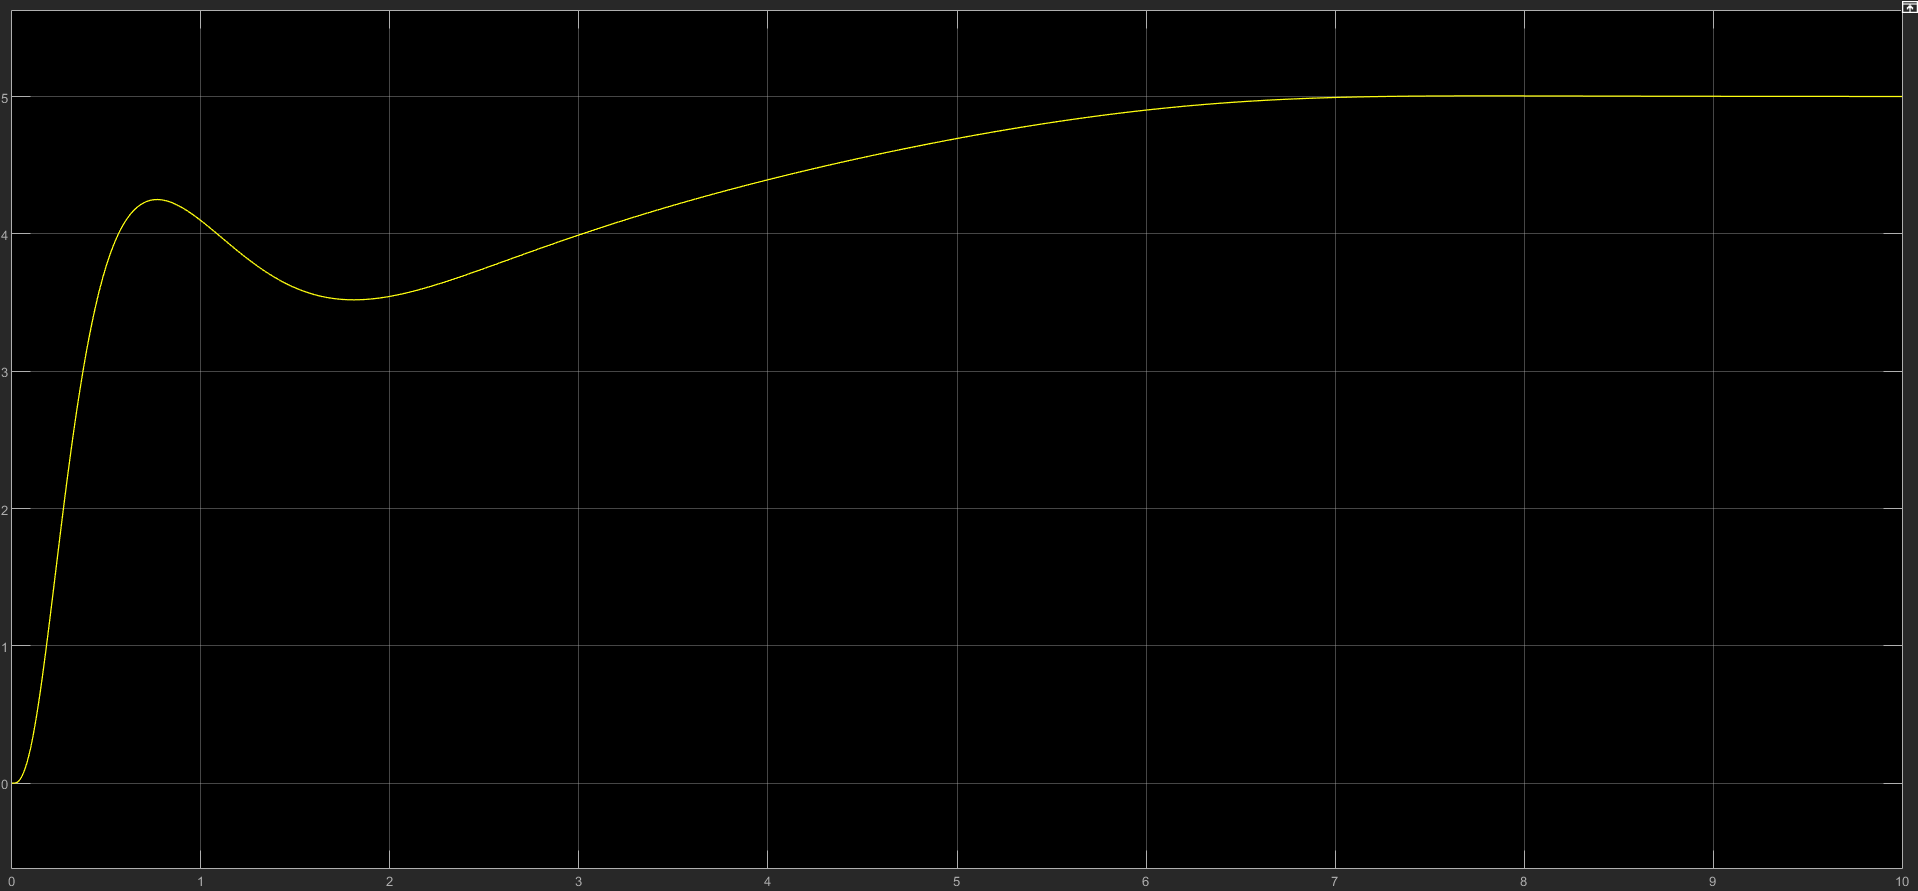
\includegraphics[width=1\linewidth]{../img/Q1_linearMPC_RES}
	\caption{پاسخ سیستم با کنترلر پیش بین خطی}
	\label{fig:q1linearmpcres}
\end{figure}

مشاهده می شود که سیستم فوق قادر است مدل را در زمان 8 ثانیه به پایداری برساند و خطای ماندگار آن صفر شود.

\subsection*{سوال سوم}
در این بخش، با اعمال اغتشاش سینوسی به سیستم، مجددا کنترلری طراحی و تنظیم می شود.
\begin{figure}
	\centering
	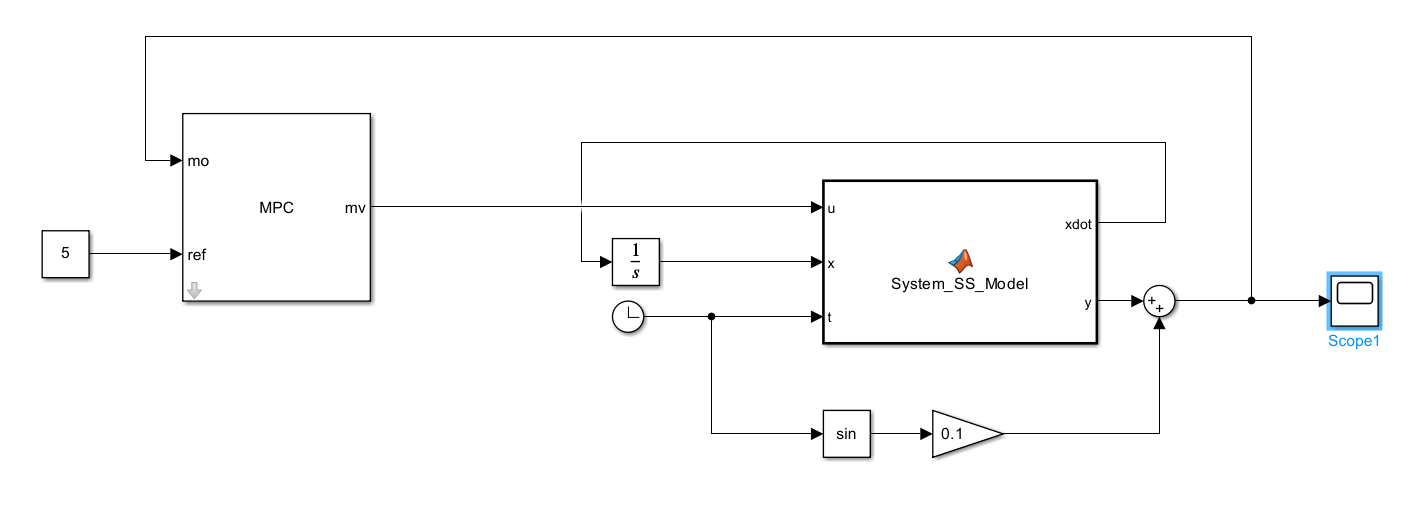
\includegraphics[width=0.7\linewidth]{../img/Q1_3_diagram}
	\caption{دیاگرام سیستم همراه با اغتشاش}
	\label{fig:q13diagram}
\end{figure}
\begin{figure}
	\centering
	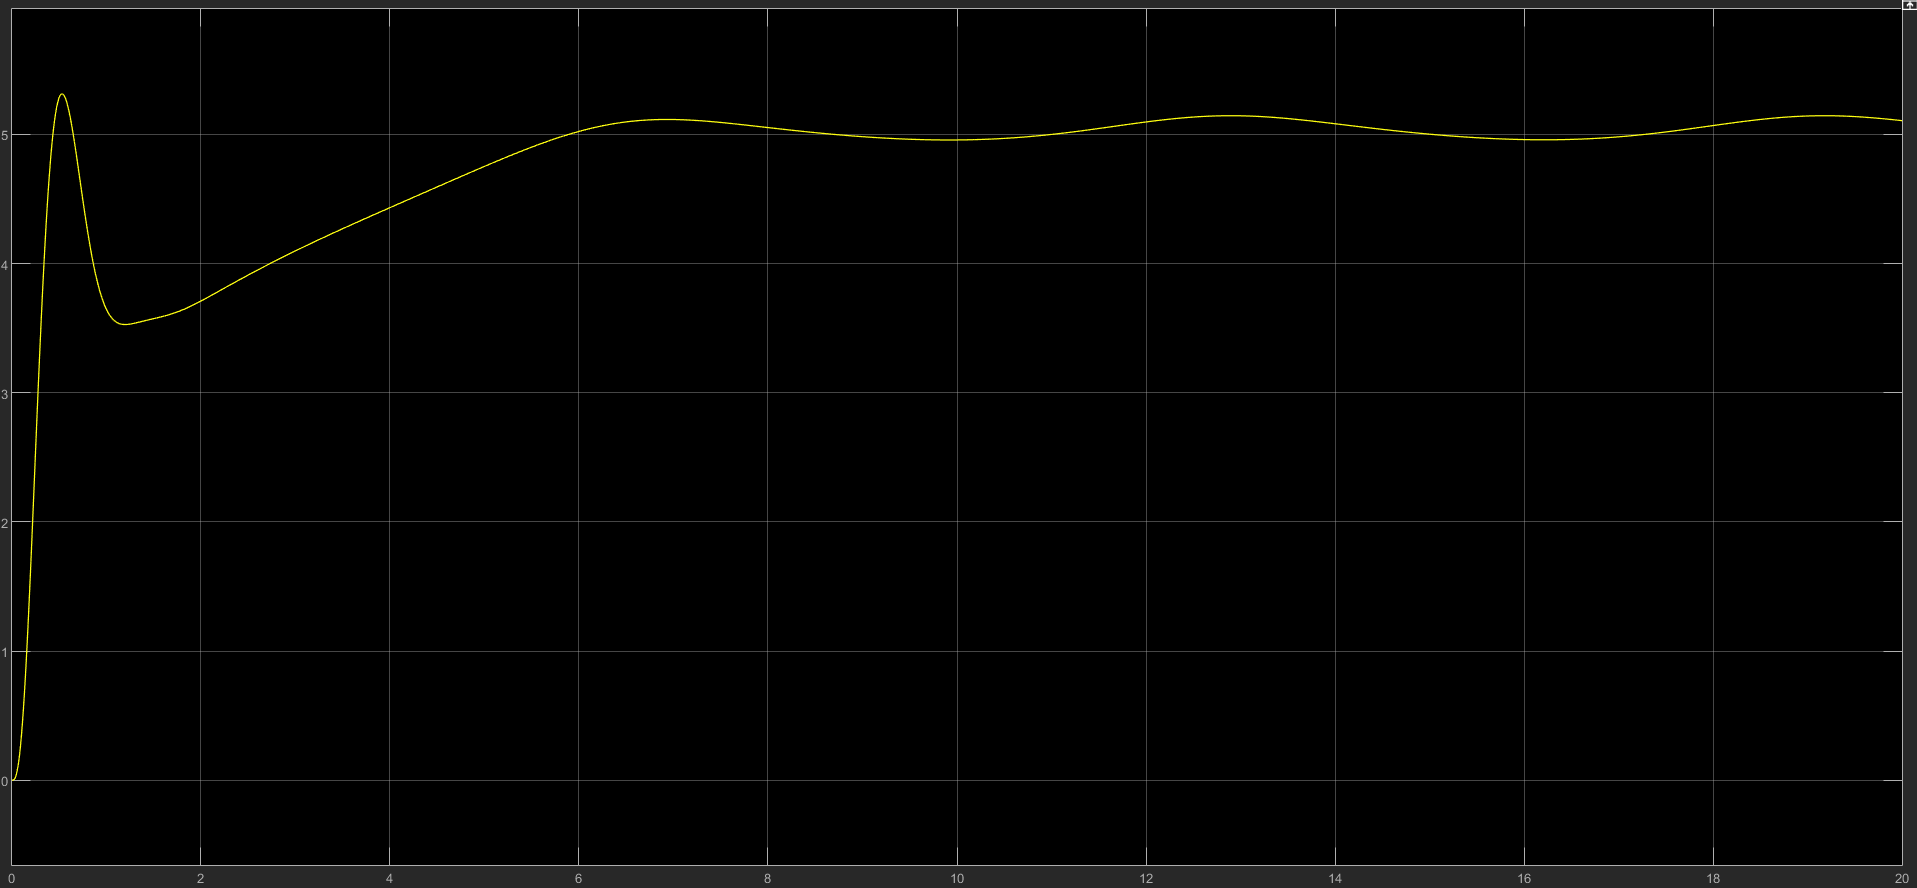
\includegraphics[width=0.7\linewidth]{../img/Q1_part3_response}
	\caption{پاسخ سیستم همراه با اغتشاش}
	\label{fig:q1part3response}
\end{figure}

مشاهده می شود که با اعمال اغتشاش به کنترلر فوق، پاسخ نهایی دارای نوسان هایی خواهد بود و این اغتشاش از سیستم حذف نشده است.
\subsection*{سوال چهارم}
در این بخش، با تغییر ساختار کنترلر به طوری که شامل یک کنترلر PID نیز باشد، سعی می کنیم تا اثر اغتشاش وارد شده به سیستم را حدف کرده و کنترلر $Tube MPC$ را تشکیل دهیم. برای این منظور، با اضافه کردن یک بلوک PID به سیستم و تنظیم ضرایب آن خواهیم داشت:
\begin{figure}[H]
	\centering
	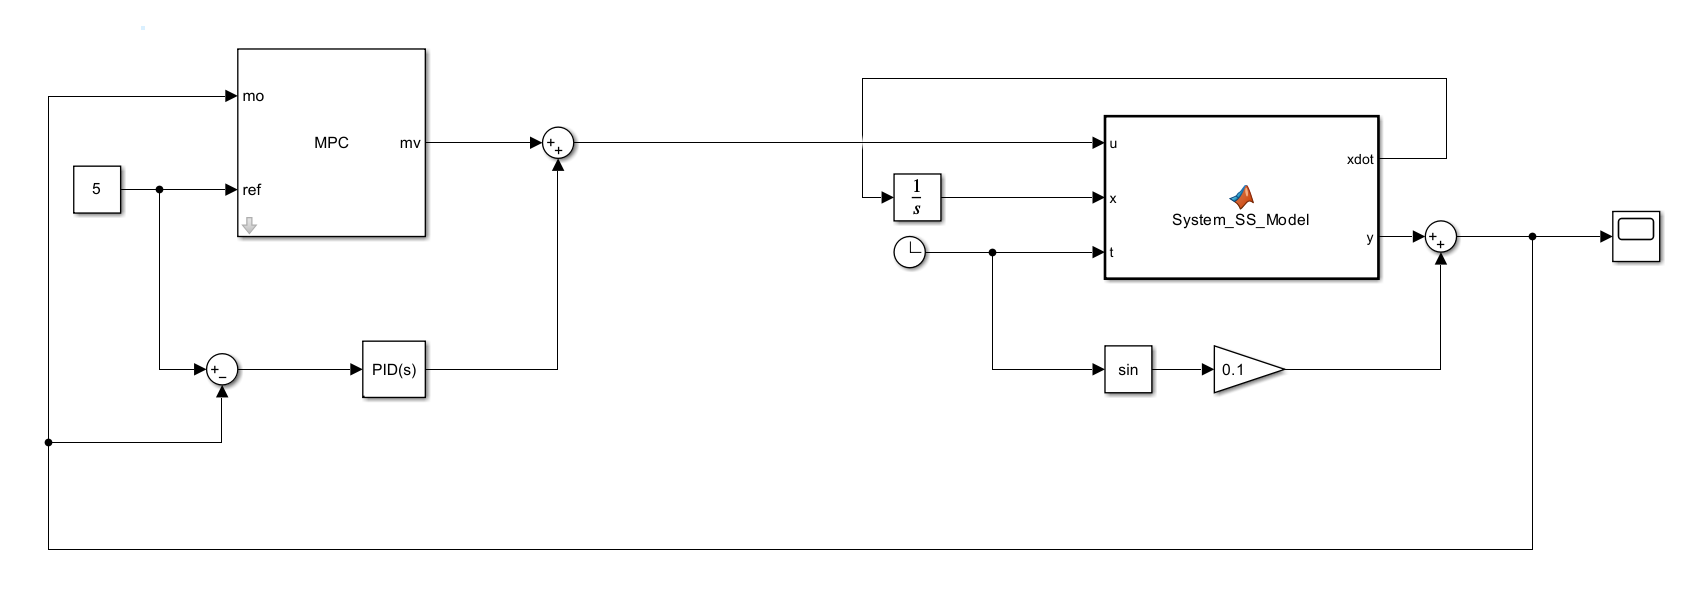
\includegraphics[width=1\linewidth]{../img/Q1_part4_diagram}
	\caption{دیاگرام سیستم $Tube MPC$}
	\label{fig:q1part4diagram}
\end{figure}
با تنظیم ضرایب PID به طوری که کنترلر بتواند با ثابت زمانی کوتاهی به تغییرات پاسخ دهد و همچنین اورشوت کمی داشته باشد تنظیم شده است.
ضرایب PID مورد استفاده در این سیستم به شرح زیر است.
\[
P = 14.05 , I = 1.12 , D = 19.04
\]
پاسخ این سیستم نسبت به ورودی قبلی به صورت زیر خواهد بود:
\begin{figure}[H]
	\centering
	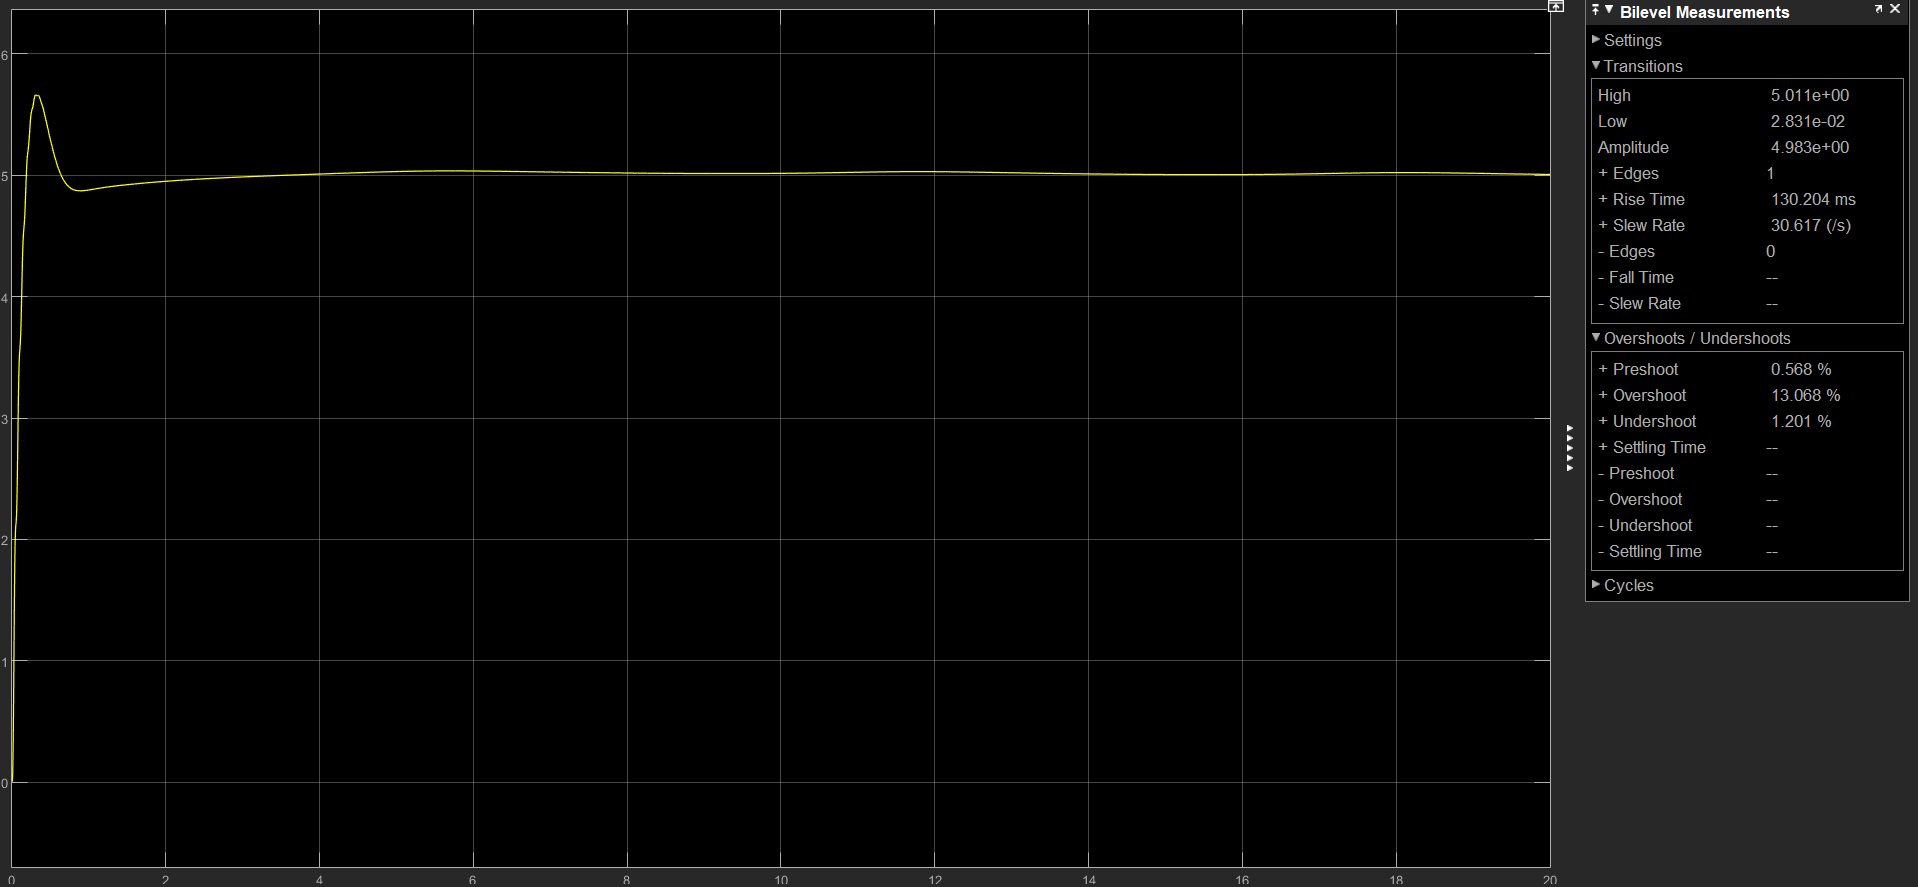
\includegraphics[width=1\linewidth]{../img/Q1_TubeMPC_Response}
	\caption{پاسخ $Tube MPC$}
	\label{fig:q1tubempcresponse}
\end{figure}
در اینجا مشاهده می شود که خطای ماندگار سیستم پس از بهینه سازی ضرایب PID، همچنان زیاد است و مقداری برابر با 13 درصد دارد که برای سیستم قابل تحمل نیست.
\subsection*{سوال پنجم}
با توجه به نتایج بخش قبل، برای کاهش میزان فراجهش، لازم است در این قسمت قیدی بر روی خروجی کنترلر اعمال شود تا از اعمال ورودی های بزرگ به سیستم خودداری شود. برای تعیین این قید، ابتدا به مشاهده و ارزیابی تلاش کنترلی کنترلر در شبیه سازی قسمت قبل می پردازیم.

\begin{figure}[H]
	\centering
	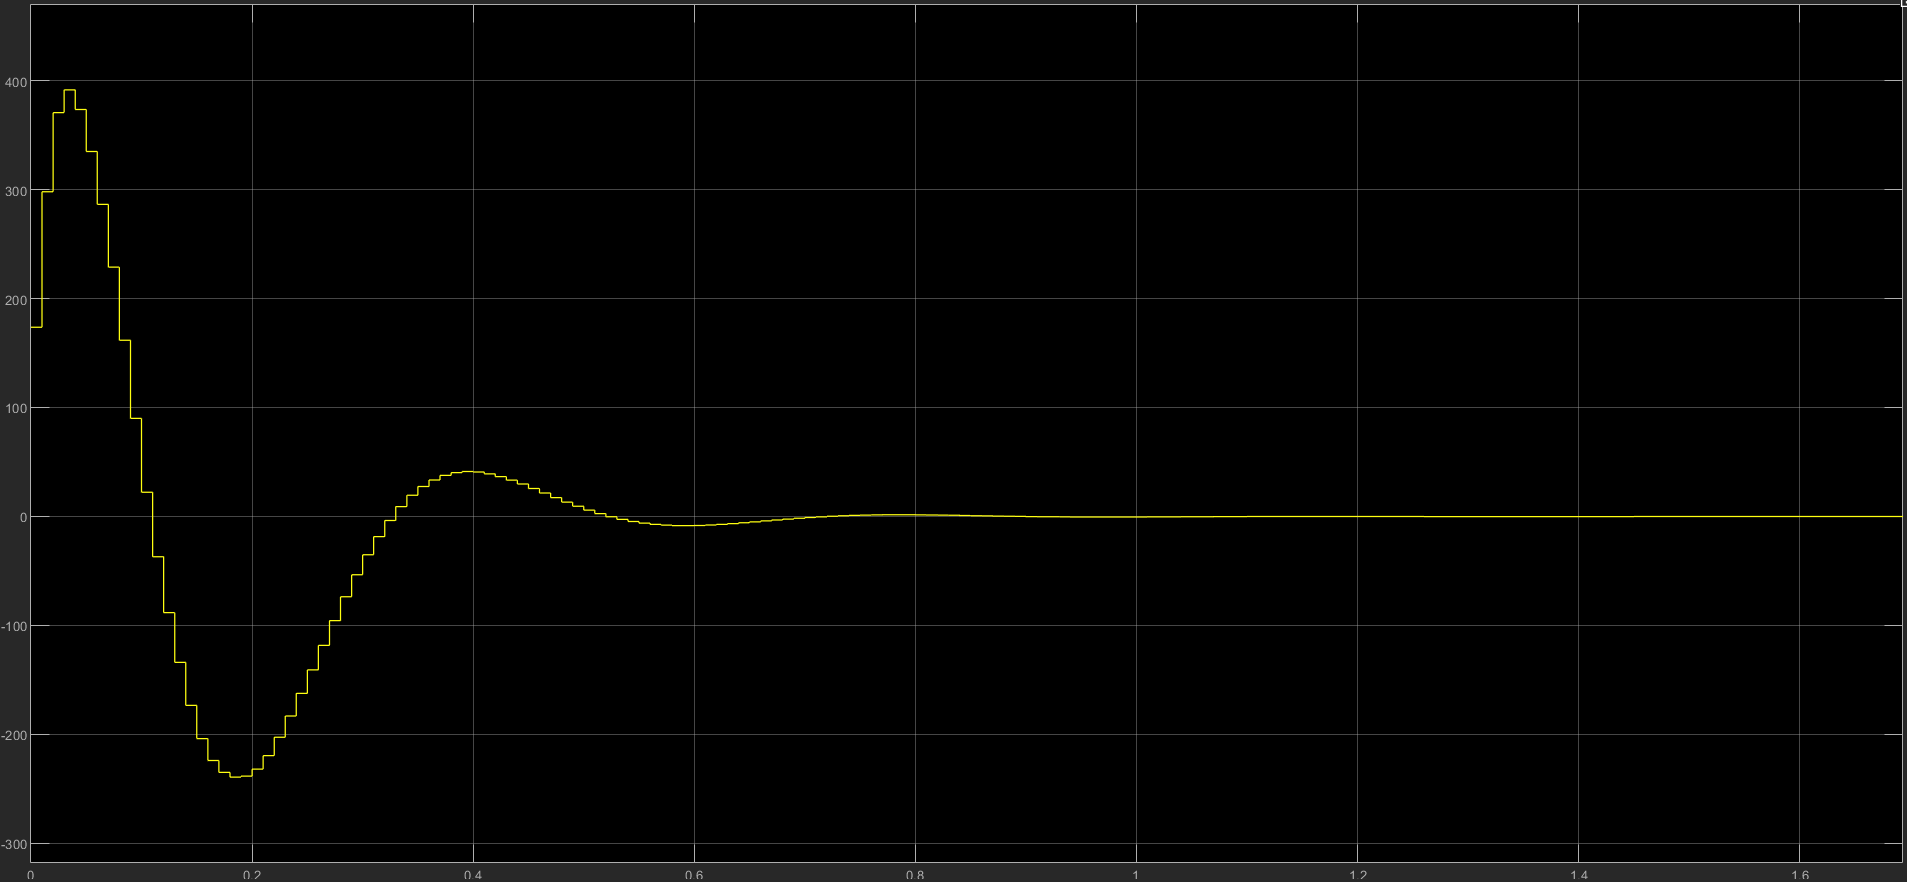
\includegraphics[width=1\linewidth]{../img/Q1_part4_Control_effort}
	\caption{تلاش کنترلی $Tube MPC$}
	\label{fig:q1part4controleffort}
\end{figure}
 
 مشاهد می شود که کنترلر فرمات های کنترلی با مقدار بیشینه ی 400 ایجاد کرده است و پس از آن، مقادیر کاهش یافته اند. با دانستن این مورد، قید هایی بر روس سیستم تنظیم شده تا بهترین نتیجه حاصل شود.
 با تنظیم مقدار فرمان کنترلی در بازه ی -10 و 10، پاسخ سیستم و تلاش کنترلی به شکل زیر به دست خواهد آمد.
\begin{figure}[H]
	\centering
	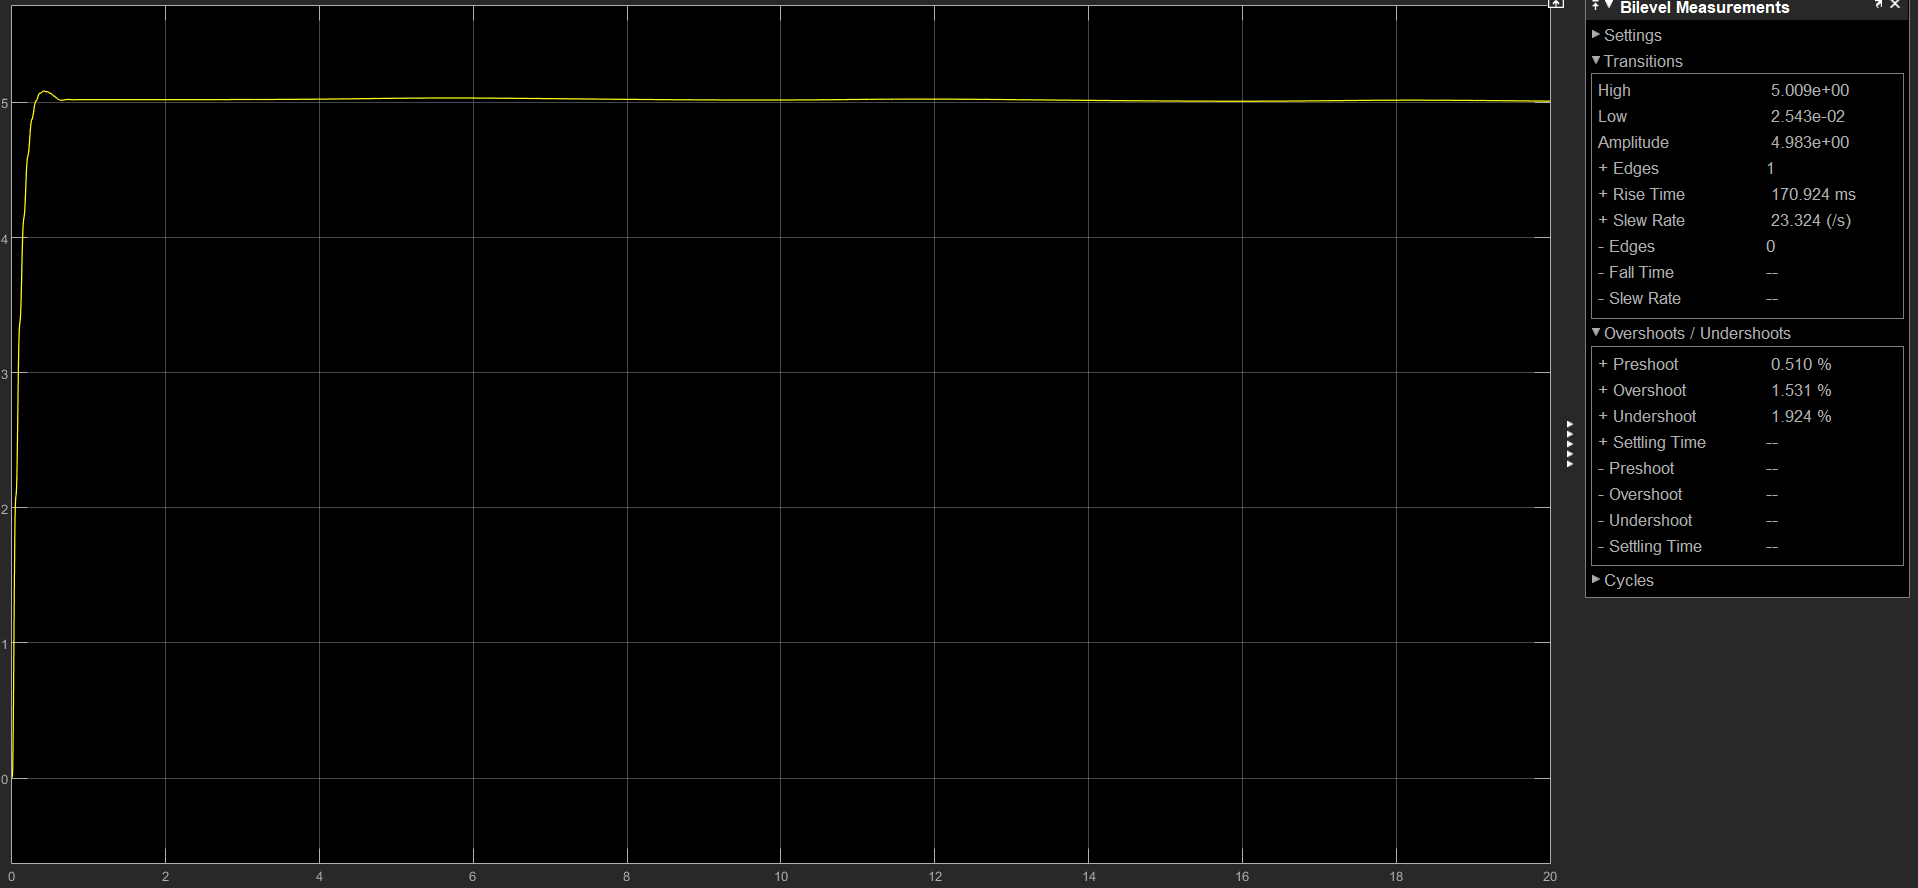
\includegraphics[width=1\linewidth]{../img/Q1_Constrained_TubeMPC_Response}
	\caption{تلاش کنترلی $Tube MPC$ مقید}
	\label{fig:q1constrainedtubempcresponse}
\end{figure}
\begin{figure}
	\centering
	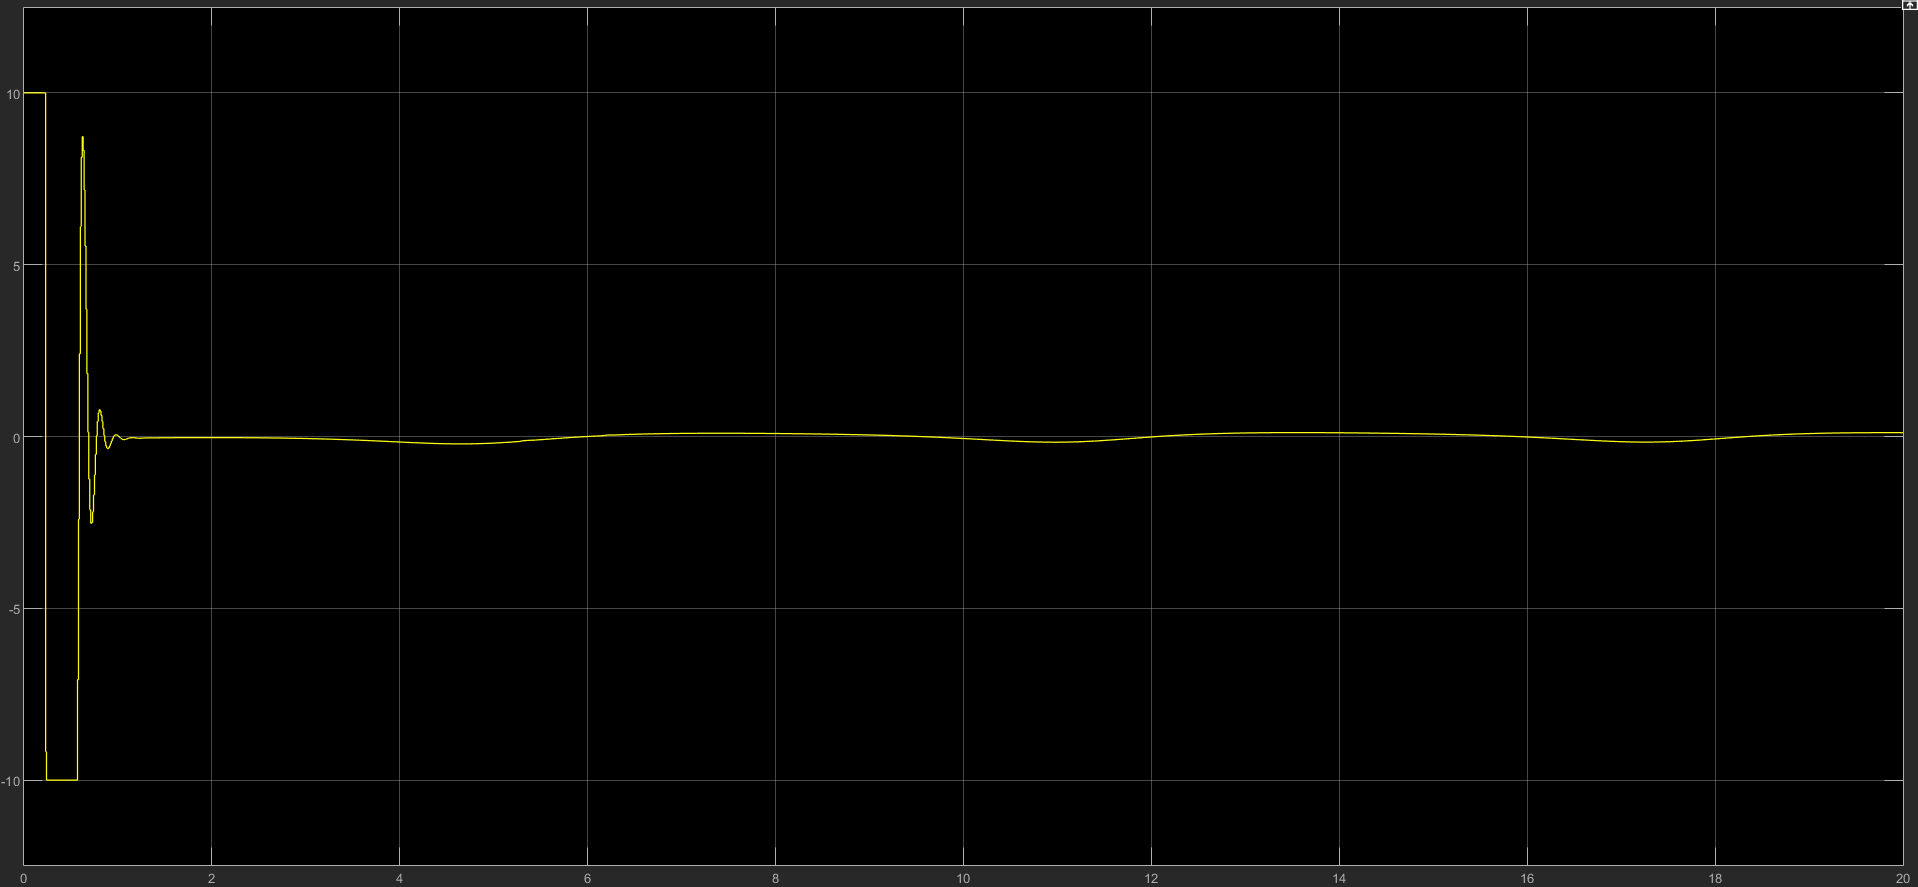
\includegraphics[width=1\linewidth]{../img/Q1_Constrained_TubeMPC_Ceffort}
	\caption{پاسخ $Tube MPC$ مقید}
	\label{fig:q1constrainedtubempcceffort}
\end{figure}

\section*{پاسخ سوال 2}
\subsection*{پاسخ بخش یکم}
در این سوال، با وجود معادلات حالت سیستم، می توان برای شبیه سازی آن را مستقیما به عنوان یک تابع در فضای سیمولینک تعریف کرد. برای این منظور، سیستمی به شکل زیر طراحی می شود.
\begin{figure}[H]
	\centering
	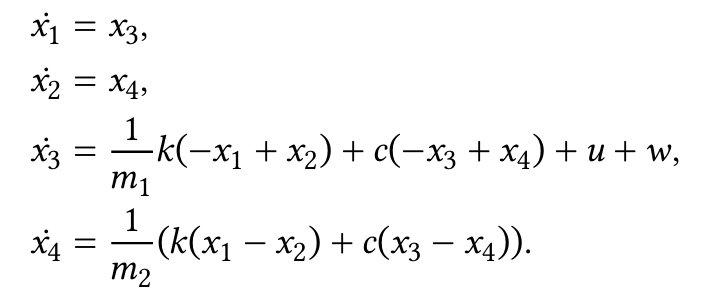
\includegraphics[width=0.7\linewidth]{../img/Q2_SS}
	\caption{معادلات حالت سیستم}
	\label{fig:q2ss}
\end{figure}
 در گام اول، سیستم مورد نظر در محیط سیمولینک تعریف شده و سپس پاسخ پله ی حلقه باز آن را بررسی می کنیم.
\begin{figure}[H]
	\centering
	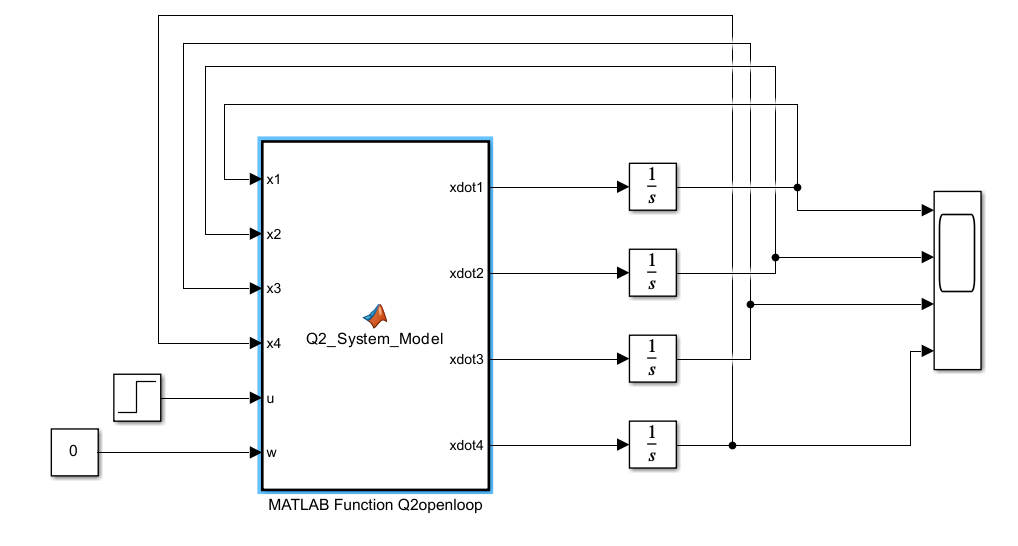
\includegraphics[width=1\linewidth]{../img/Q2_openloop_diagram}
	\caption{دیاگرام سیستم حلقه باز}
	\label{fig:q2openloopdiagram}
\end{figure}
\begin{figure}[H]
	\centering
	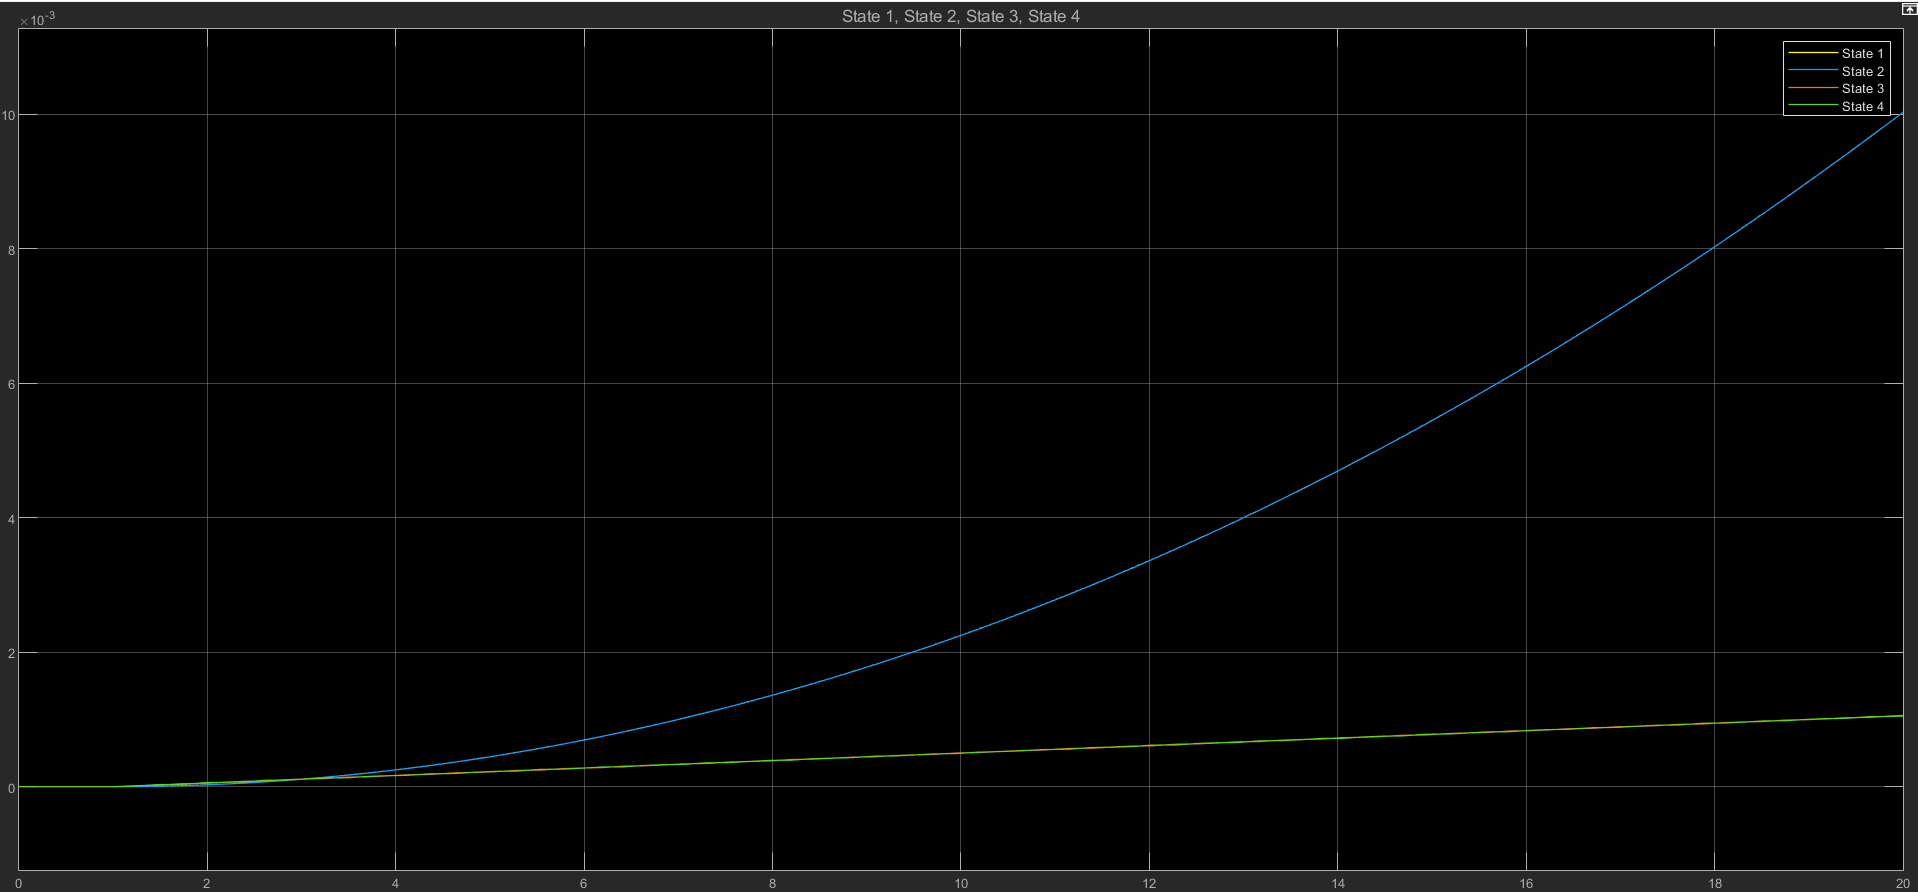
\includegraphics[width=1\linewidth]{../img/Q2_openloop_response}
	\caption{پاسخ پله ی حلقه باز}
	\label{fig:q2openloopresponse}
\end{figure}
مشاهده می شود که حالت های این سیستم به طور حلقه باز پایدار نیستند.
در ادامه با پیاده سازی یک کنترلر پیش بین خطی، سعی بر کنترل این سیستم خواهیم کرد. دیاگرام این سیستم به صورت زیر خواهد بود.
\begin{figure}[H]
	\centering
	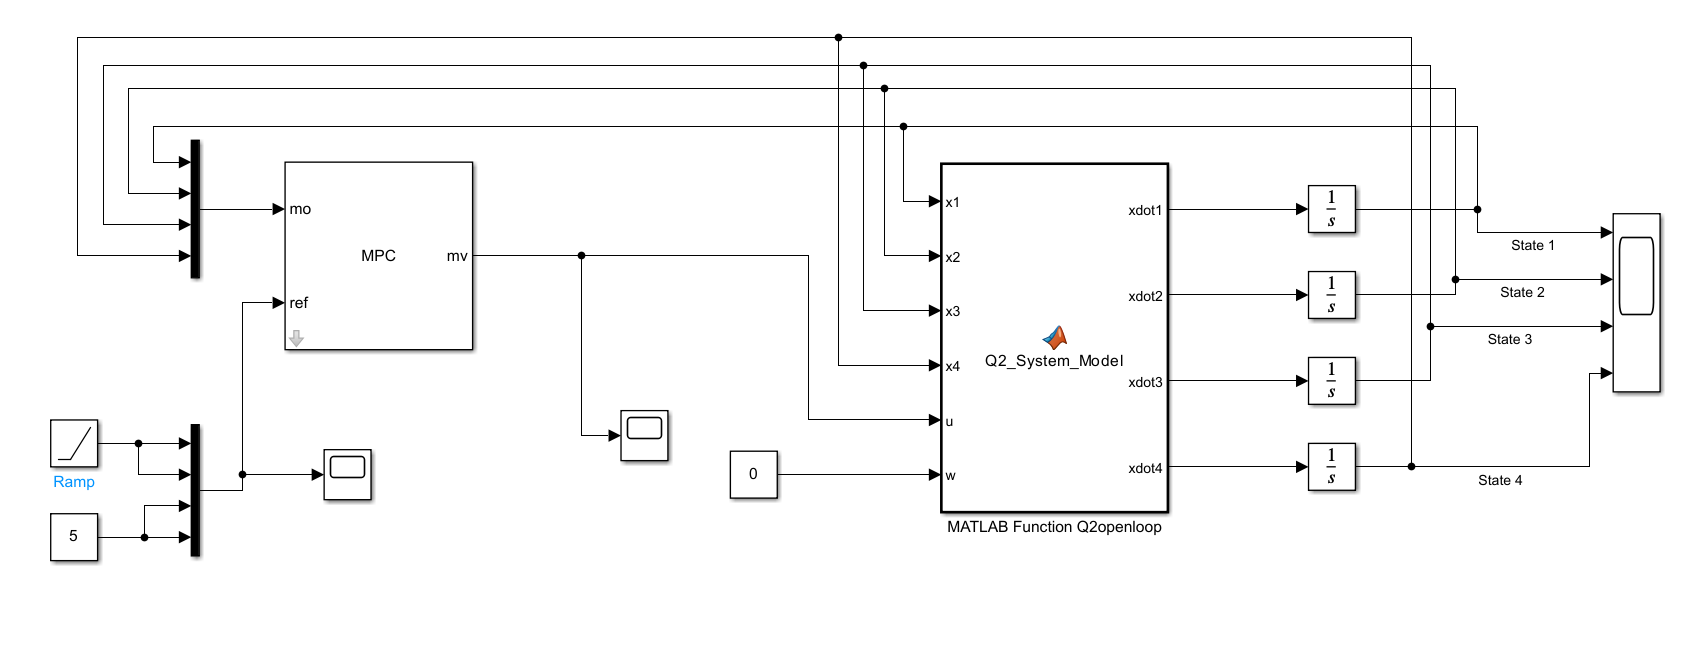
\includegraphics[width=1\linewidth]{../img/Q2_LMPC_diagram}
	\caption{دیاگرام سیستم}
	\label{fig:q2lmpcdiagram}
\end{figure}
برای تنظیم کنترلر پیش بین، از نرخ نمونه برداری $ 0.01 $ ثانیه، افق پیش بین 650 و افق کنترلی 100 استفاده شده است. پاسخ سیستم به ورودی های تعیین شده به صورت زیر به دست خواهد آمد

\begin{figure}[H]
	\centering
	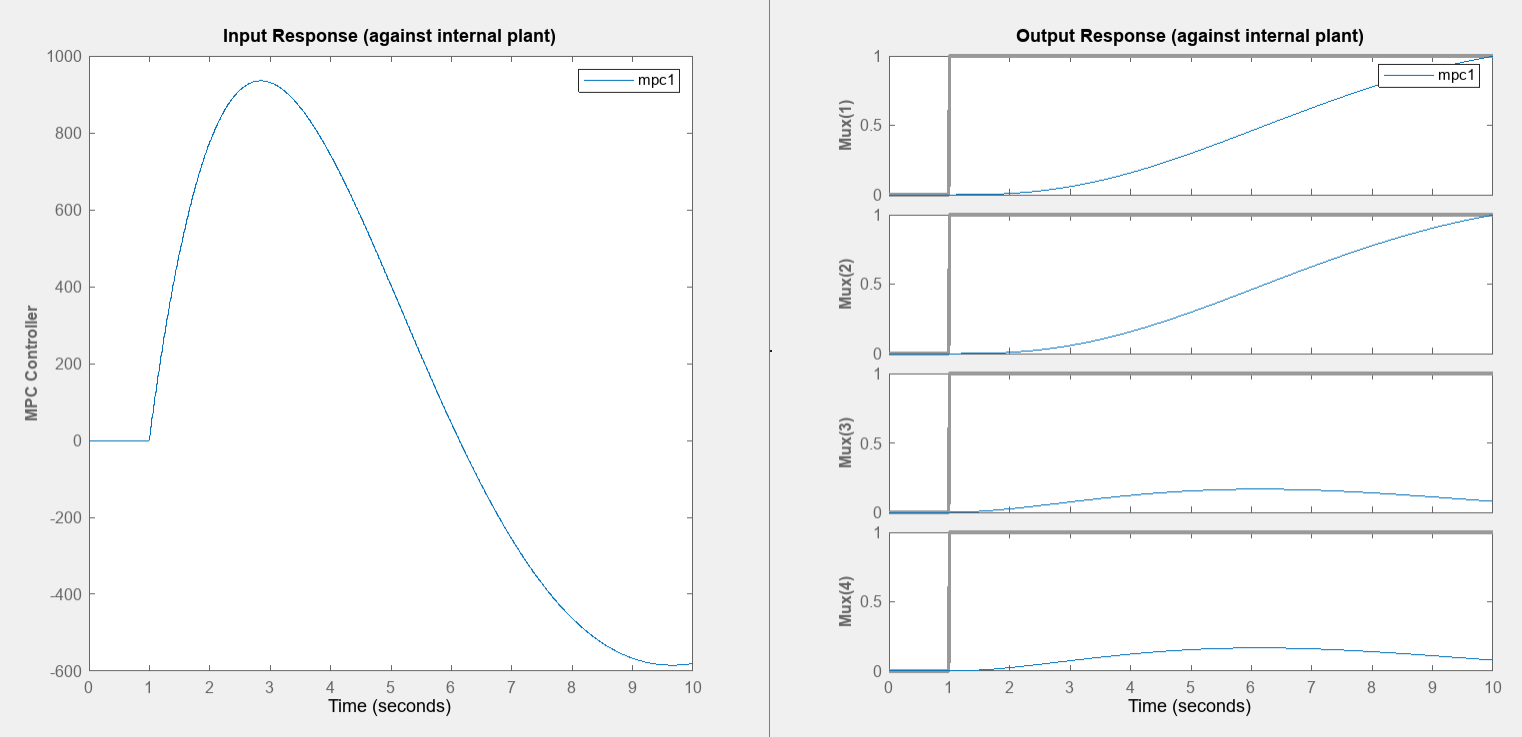
\includegraphics[width=1\linewidth]{../img/Q2_LMPC_ِDesign}
	\caption{پارامتر های کنترلر MPC}
	\label{fig:q2lmpcdesign}
\end{figure}

\begin{figure}[H]
	\centering
	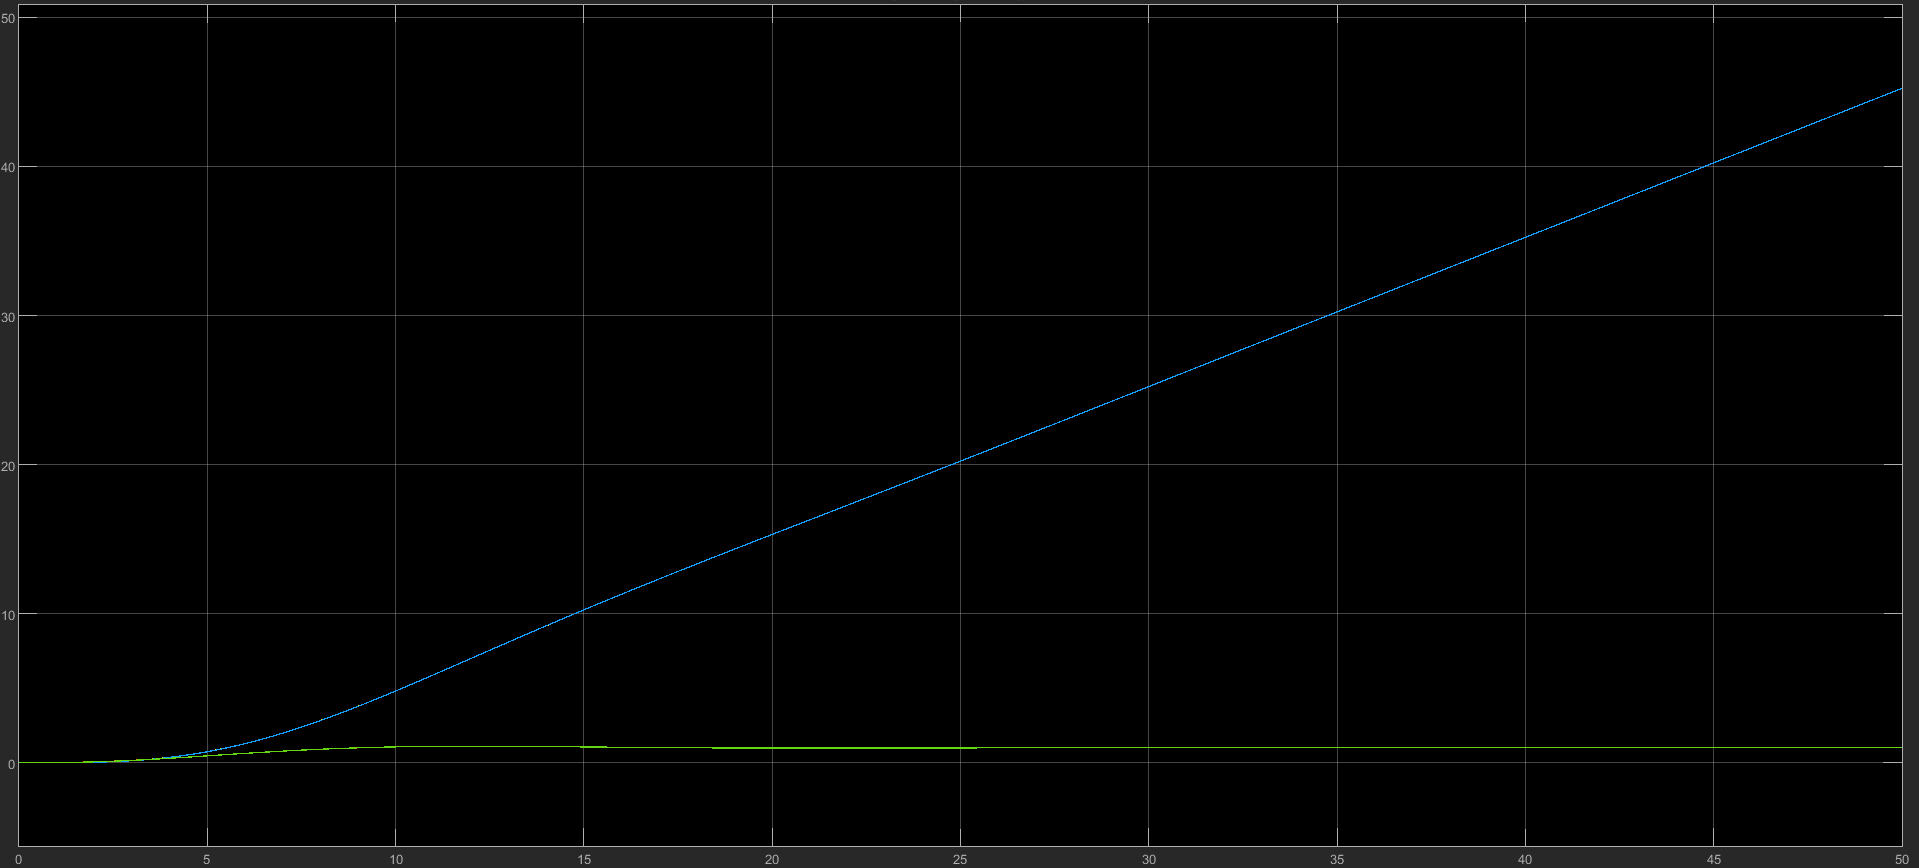
\includegraphics[width=1\linewidth]{../img/Q2_LMPC_Response}
	\caption{پاسخ سیستم با کنترلر پیش بین خطی}
	\label{fig:q2lmpcresponse}
\end{figure}
با مشاهده ی پاسخ این سیستم متوجه می شویم که کنترلر حالت های اول و دوم را به خوبی کنترل کرده و خروجی، ورودی را دنبال می کند. اما برای حالت های سوم و چهارم، این اتفاق نمی افتد و مقدار خروجی با ورودی فاصله ی زیادی دارد.
همچنین، نمودار خروجی کنترلر به صورت زیر است:
\begin{figure}[H]
	\centering
	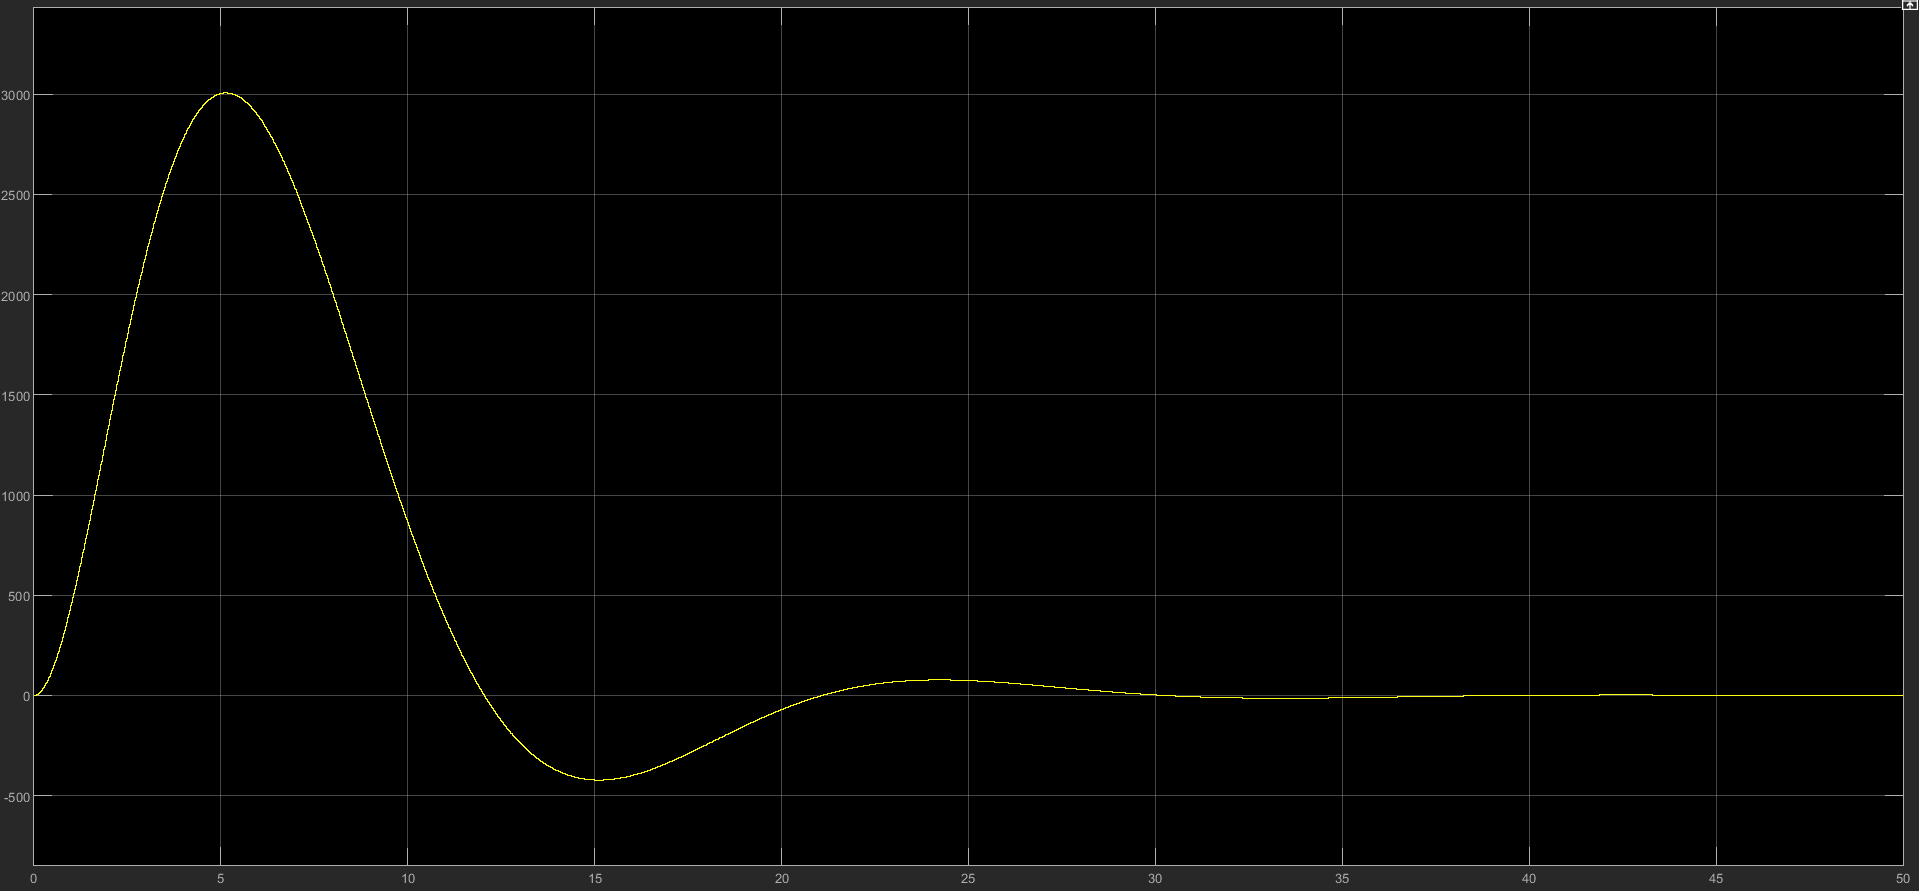
\includegraphics[width=1\linewidth]{../img/Q2_LMPC_ِCeffort}
	\caption{نمودار تلاش کنترلی}
	\label{fig:q2lmpcceffort}
\end{figure}
آنچنان که مشاهده می شود، مقدار فرمان کنترلی بسیار بزرگ است. برای جلوگیری از این کار و نرمالایز کردن کنترلر، می توان از بلوک های بهره برای افزایش مقادیر کنترلر استفاده کرد.
\subsection*{پاسخ بخش دوم}
\subsubsection{قسمت اول - قید نرم}
در این بخش، با اعمال یک قید نرم برای حالت چهارم، خروجی های سیستم را مجددا بررسی می کنیم.
\begin{figure}
	\centering
	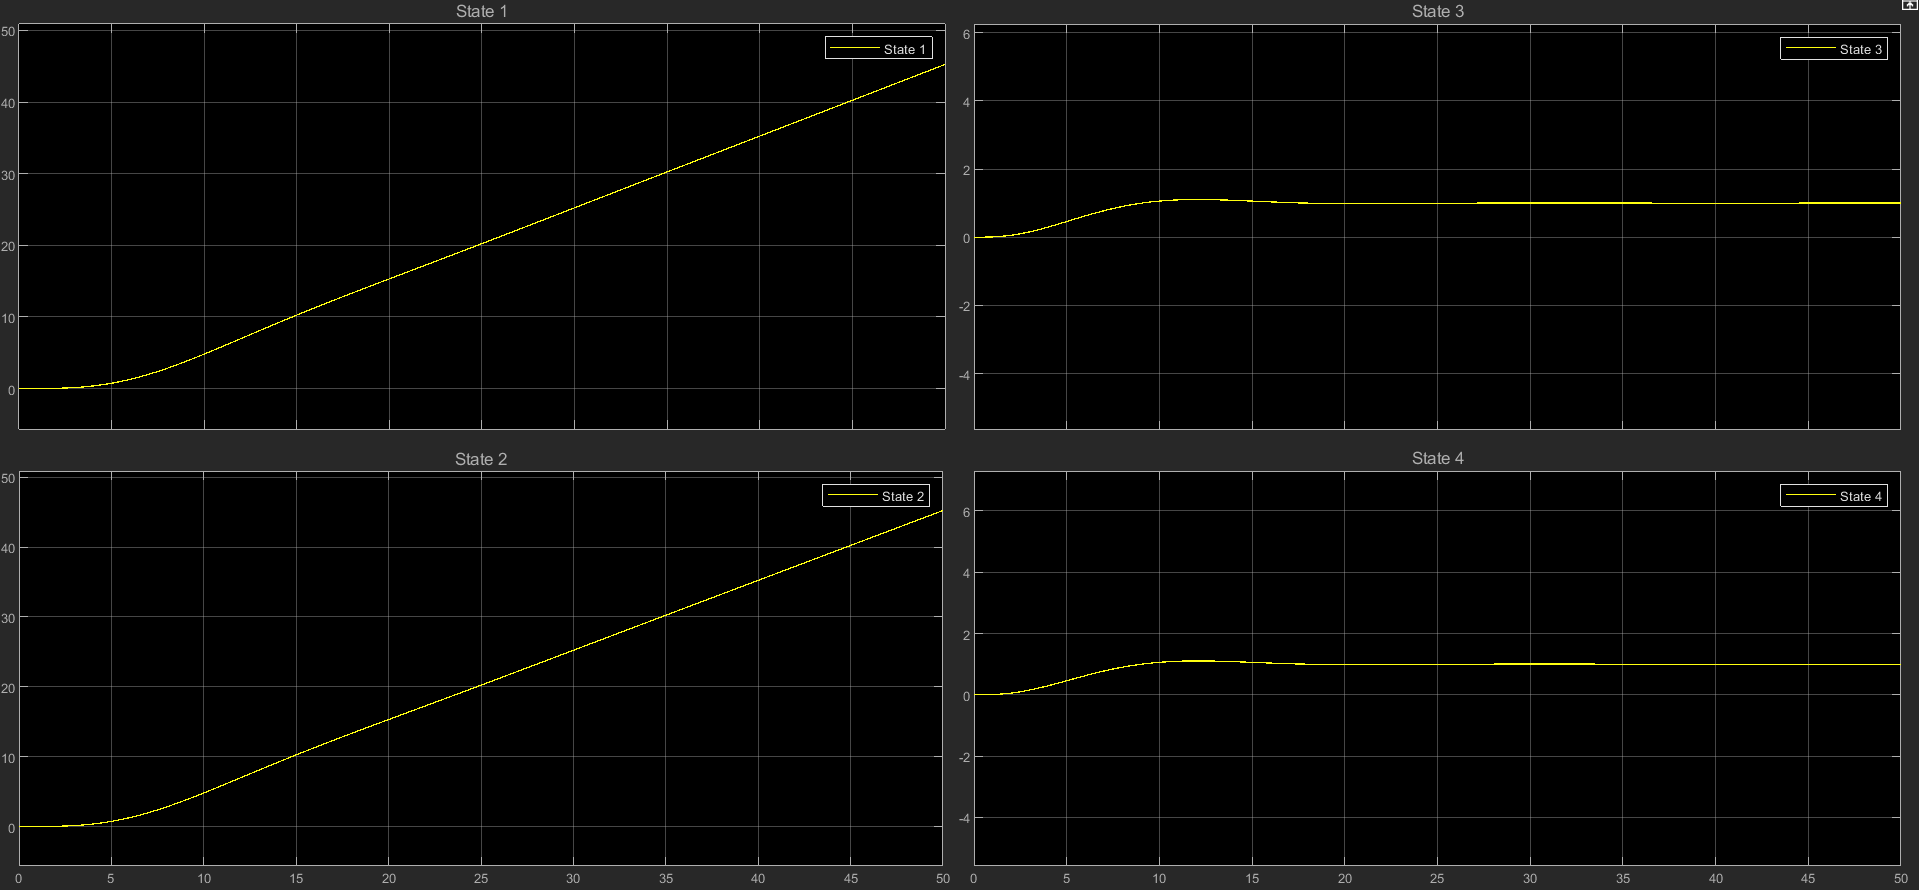
\includegraphics[width=1\linewidth]{../img/Q2_LMPC_ِsoft_Response}
	\caption{پاسخ سیستم با قید نرم}
	\label{fig:q2lmpcsoftresponse}
\end{figure}
\begin{figure}[H]
	\centering
	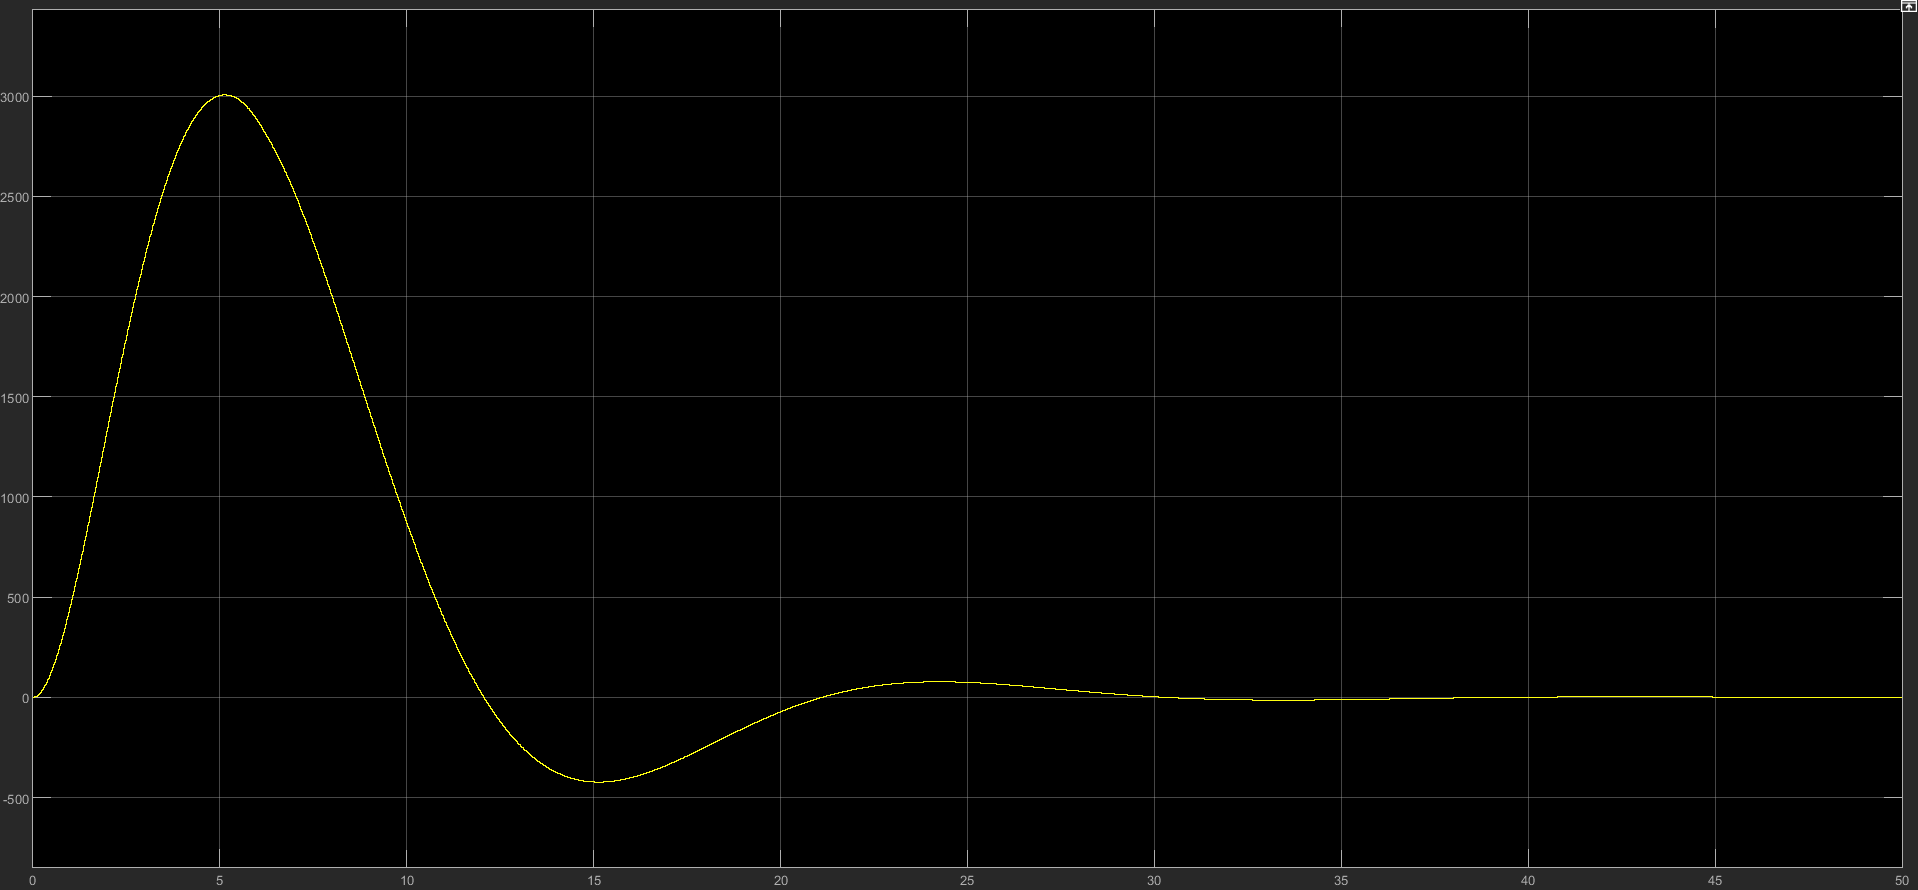
\includegraphics[width=1\linewidth]{../img/Q2_LMPC_ِsoft_Ceffort}
	\caption{تلاش کنترلی}
	\label{fig:q2lmpcsoftceffort}
\end{figure}
\begin{figure}[H]
	\centering
	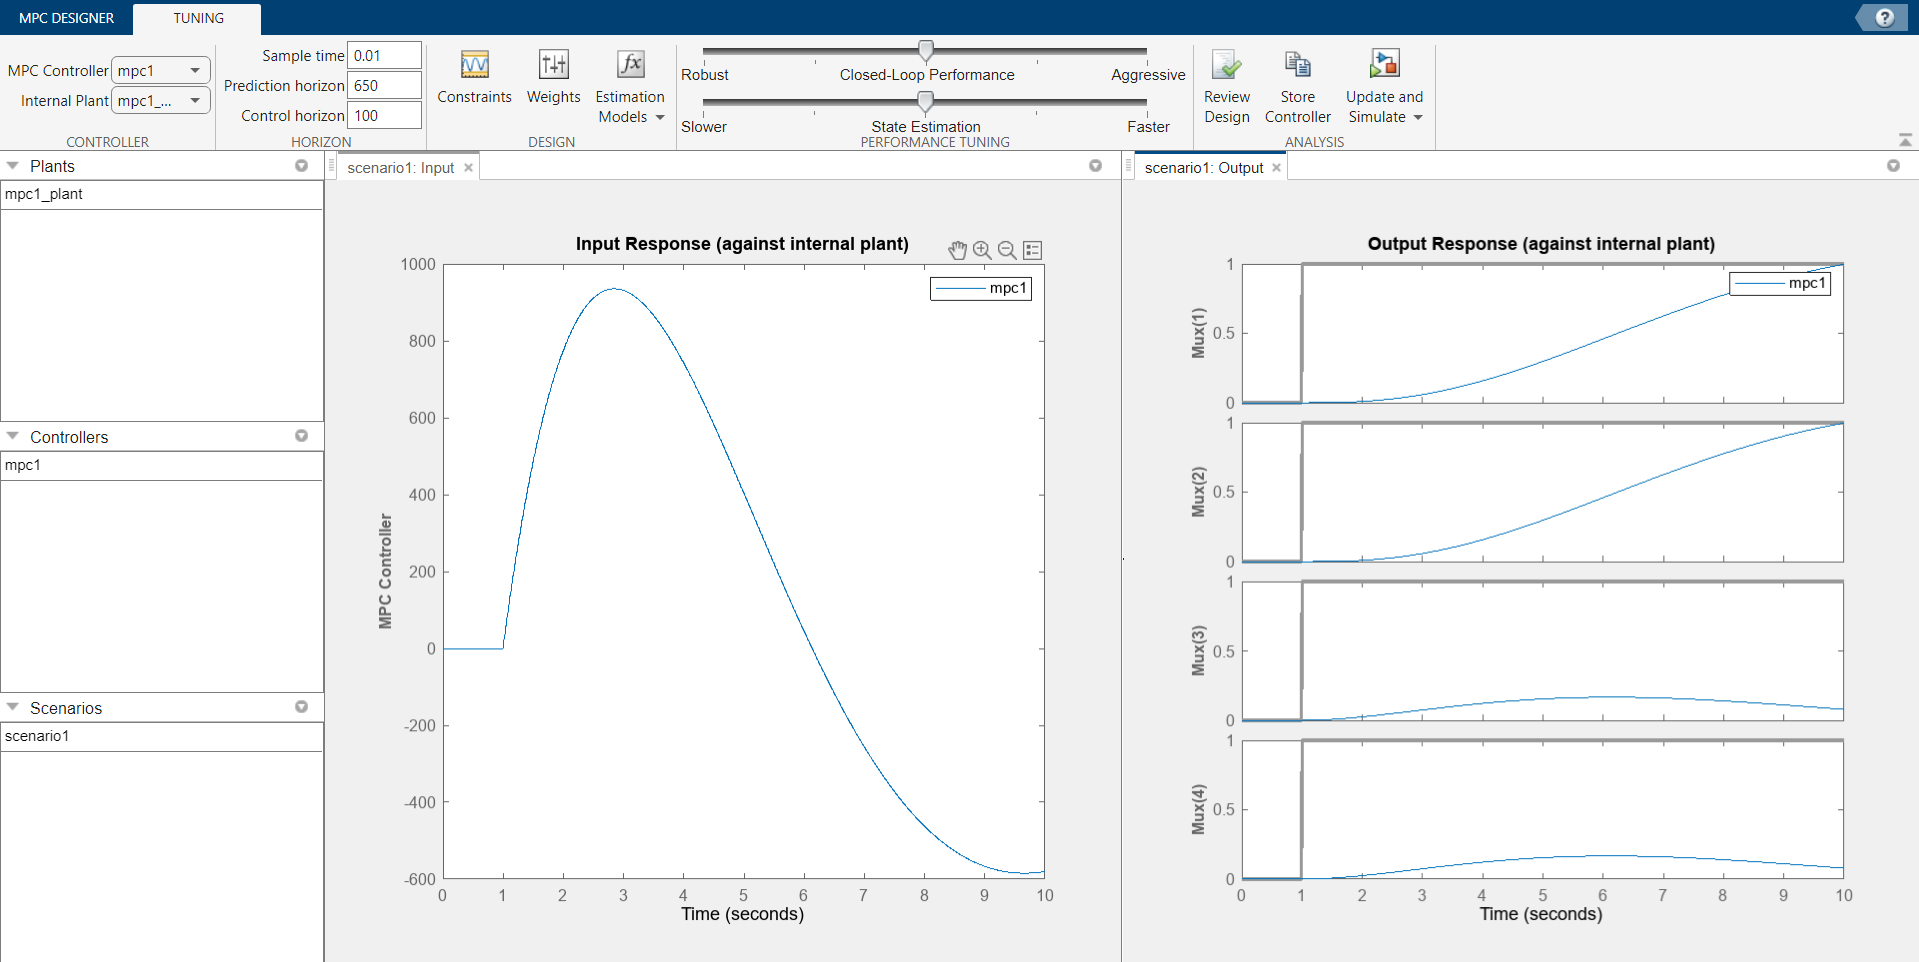
\includegraphics[width=1\linewidth]{../img/Q2_LMPC_ِsoft_setting}
	\caption{ورودی ها و خروجی ها}
	\label{fig:q2lmpcsoftsetting}
\end{figure}
\begin{figure}[H]
	\centering
	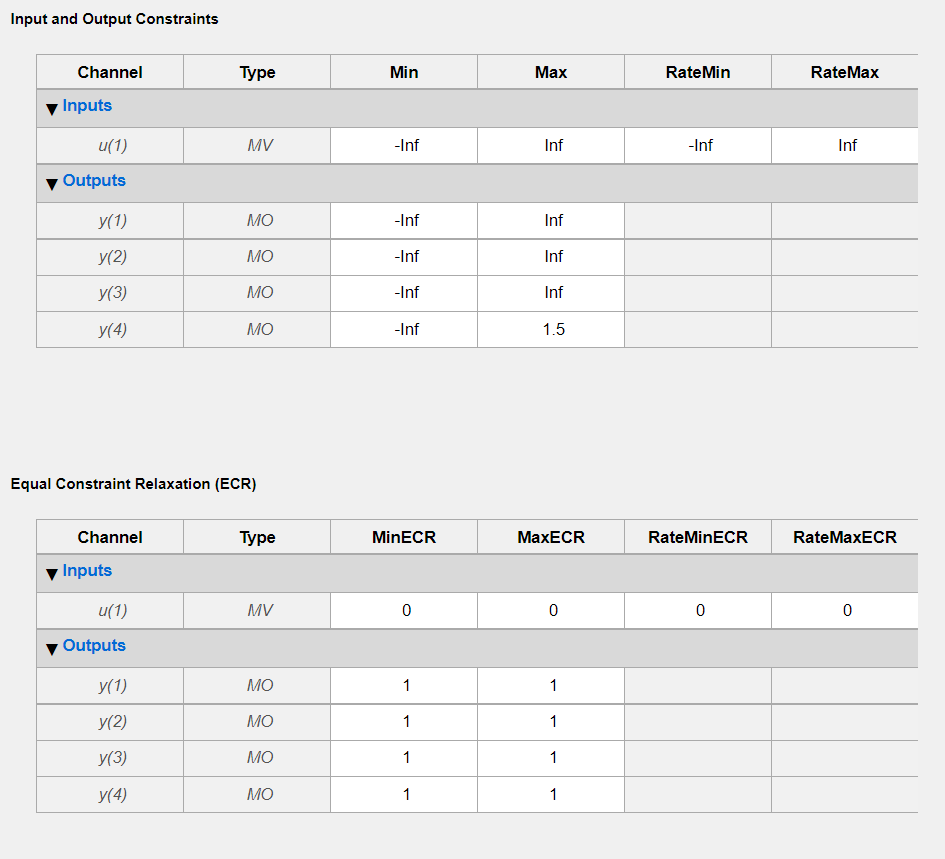
\includegraphics[width=0.7\linewidth]{../img/Q2_LMPC_ِsoft_setting1}
	\caption{تنظیمات قید ها}
	\label{fig:q2lmpcsoftsetting1}
\end{figure}
\subsubsection*{قسمت دوم - قید سخت}
حال در این بخش، با تغییر قید تعیین شده از حالت نرم به سخت، مجددا نتایج را بررسی می کنیم.
\begin{figure}[H]
	\centering
	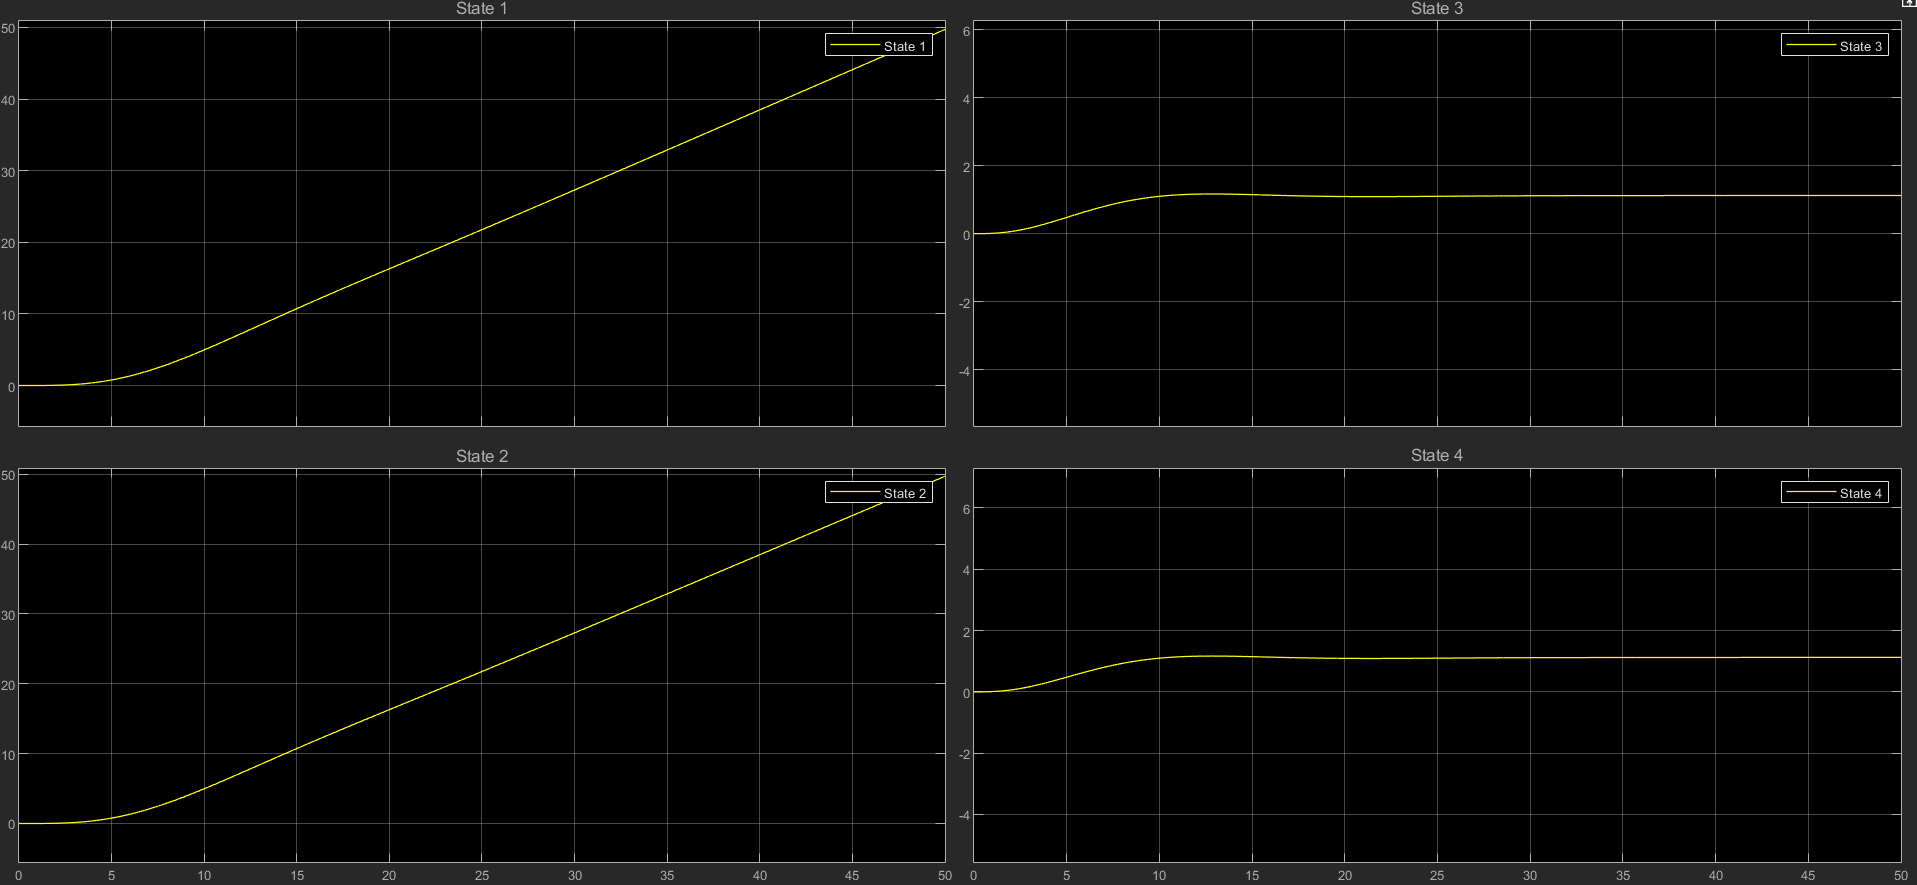
\includegraphics[width=1\linewidth]{../img/Q2_LMPC_ِHard_Response}
	\caption{پاسخ سیستم}
	\label{fig:q2lmpchardresponse}
\end{figure}
\begin{figure}[H]
	\centering
	\includegraphics[width=0.7\linewidth]{"../img/Q2_LMPC_ِHard_Ceffort"}
	\caption{تلاش کنترلی}
	\label{fig:q2lmpchardceffort}
\end{figure}
\begin{figure}[H]
	\centering
	\includegraphics[width=0.7\linewidth]{"../img/Q2_LMPC_ِHard_Ceffort"}
	\caption{تنظیمات قید های سیستم}
	\label{fig:q2lmpchardsetting}
\end{figure}
با توجه به نتایح این قسمت و بخش پیشین، مشاهده می شود که تفات چندانی میان این دو روش وجود ندارد. علت این امر آن است که کنترلر در بخش ابتدایی توانسه با حداقل تلاش کنترلی، خروجی را کنترل کند و بنابراین نیازی به اعمال ورودی های بزرگ به سیستم نبوده. بنابراین، این سیستم در حالت عادی در حیطه ی قیدها قرار می گیرد و نیازی به تلاش مضاعف کنترلر و یا محدود کردن بازه های عملکردی آن نخواهد بود.
\subsection*{پاسخ بخش سوم}
در این بخش، با اعمال یک اغتشاش سینوسی به صورت زیر، عملکرد کنترلر را مورد بررسی قرار می دهیم. برای پیاده سازی این اغتشاش در محیط سیمولینک، از یک Function Block استفاده شده است.
\begin{figure}[H]
	\centering
	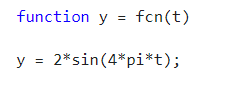
\includegraphics[width=0.7\linewidth]{../img/Q3_Disturbance}
	\caption{کد اغتشاش}
	\label{fig:q3disturbance}
\end{figure}
\begin{figure}[H]
	\centering
	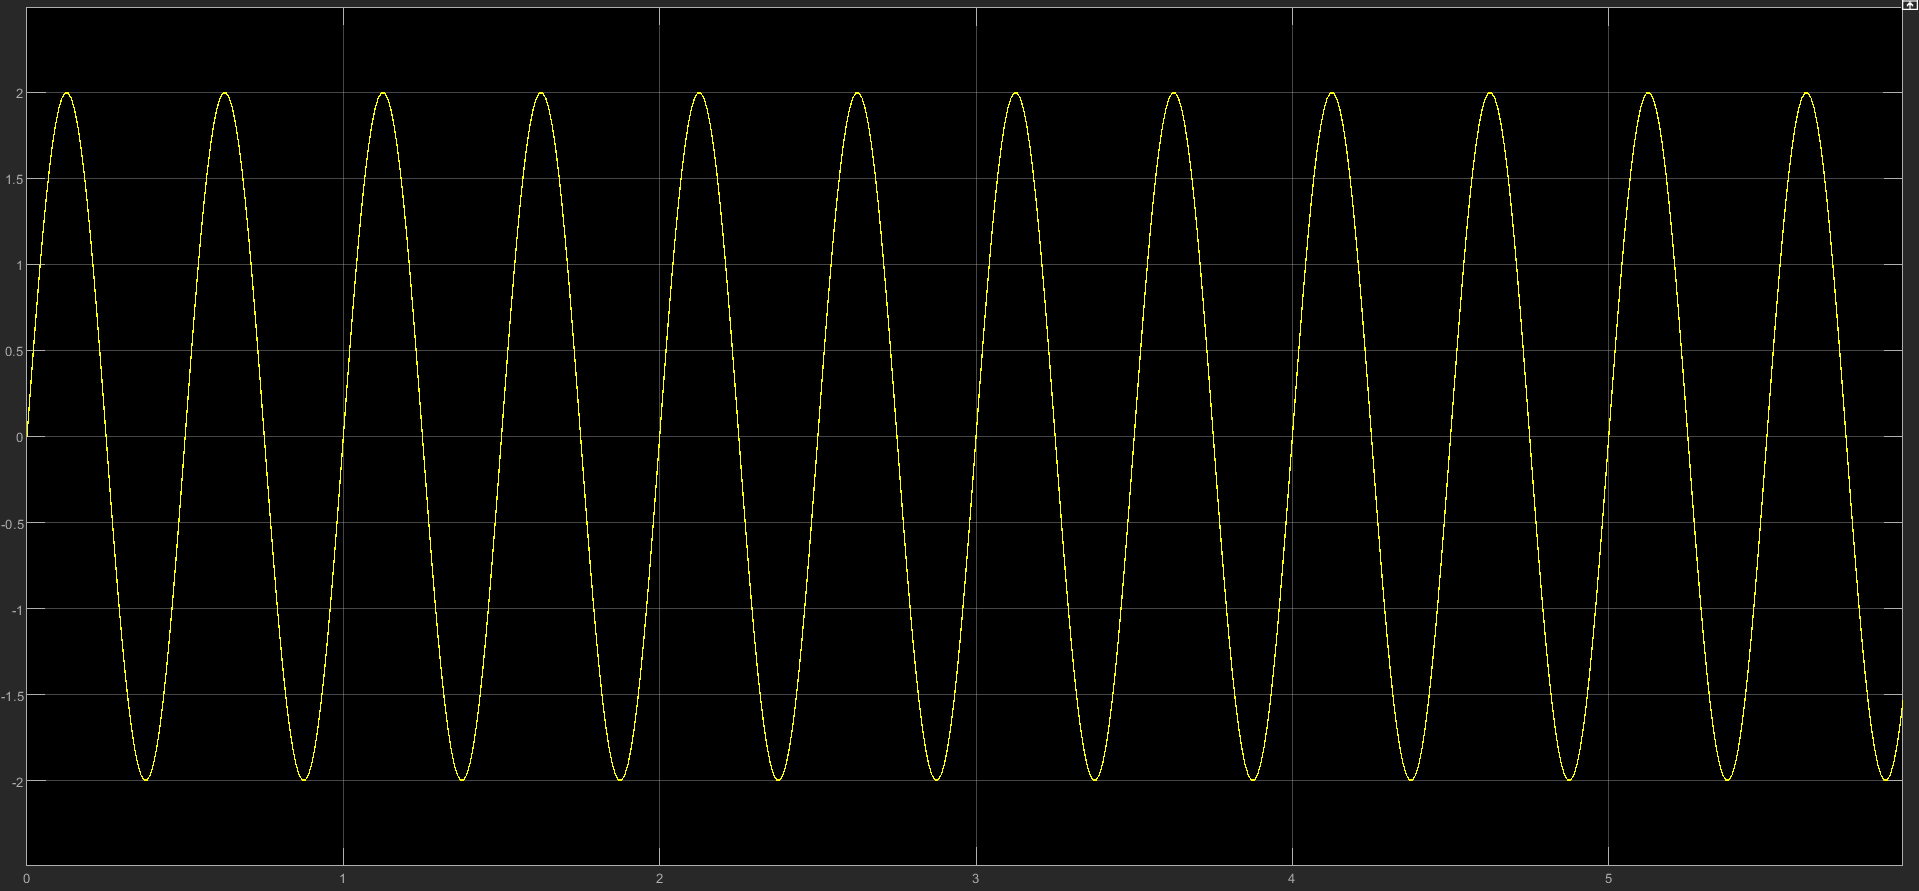
\includegraphics[width=0.7\linewidth]{../img/Q3_Disturbance_plot}
	\caption{نمودار اغتشاش}
	\label{fig:q3disturbanceplot}
\end{figure}
\begin{figure}[H]
	\centering
	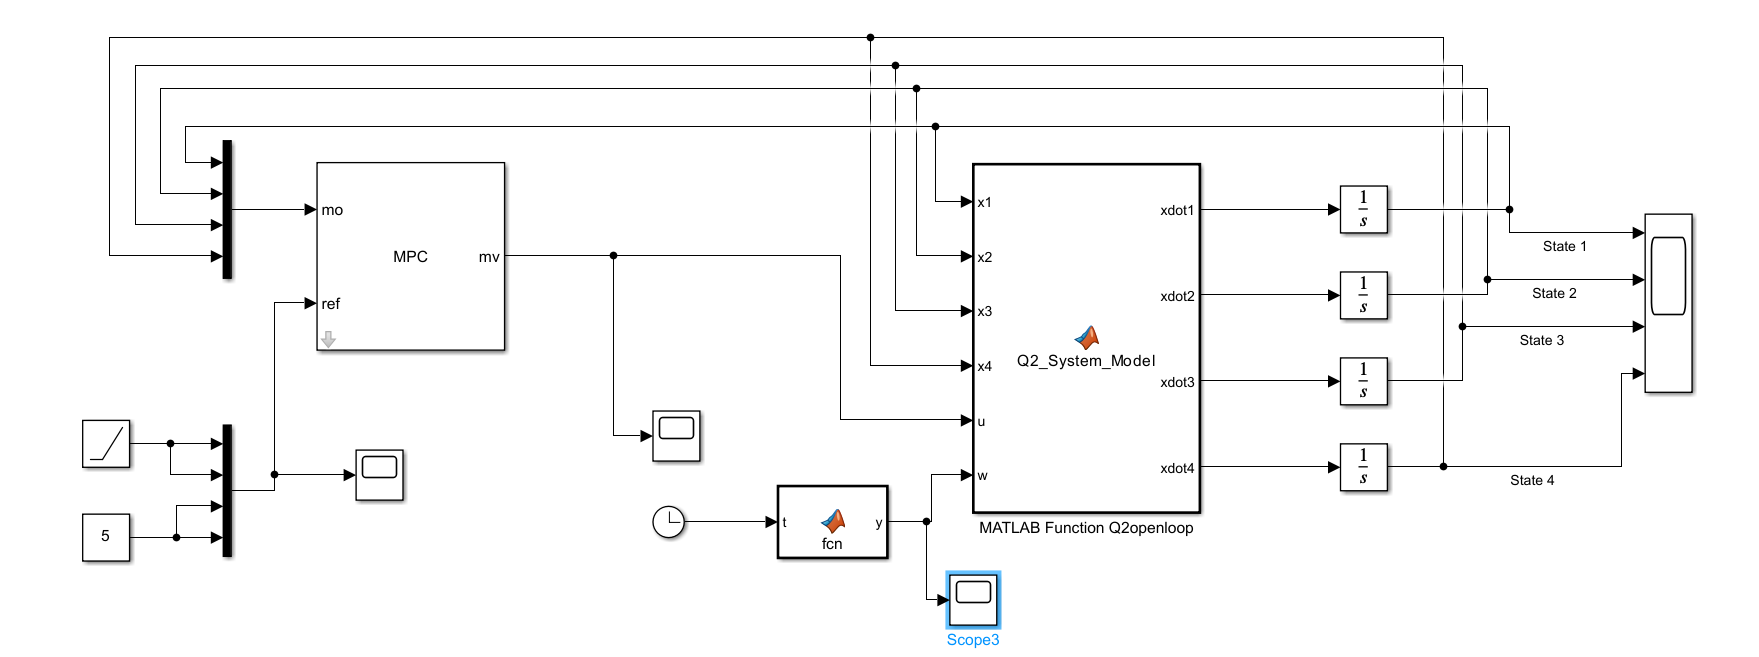
\includegraphics[width=1\linewidth]{../img/Q3_Diagram}
	\caption{دیاگرام سیستم با اغتشاش}
	\label{fig:q3diagram}
\end{figure}
به دلیل کوچک بودن مقدار اغتشاش ذکر شده در صورت سوال و قابل صرف نظر بودن از آن مقدار، در ادامه ی این آزمایش مقدار اغتشاش با دامنه ی 400 در نظر گرفته شده است تا یتوان نمایش بهتری از نمودار حاصل داشت.
در اینجا، خروچی سیستم را با این اغتشاش مشاهده می کنیم.
\begin{figure}[H]
	\centering
	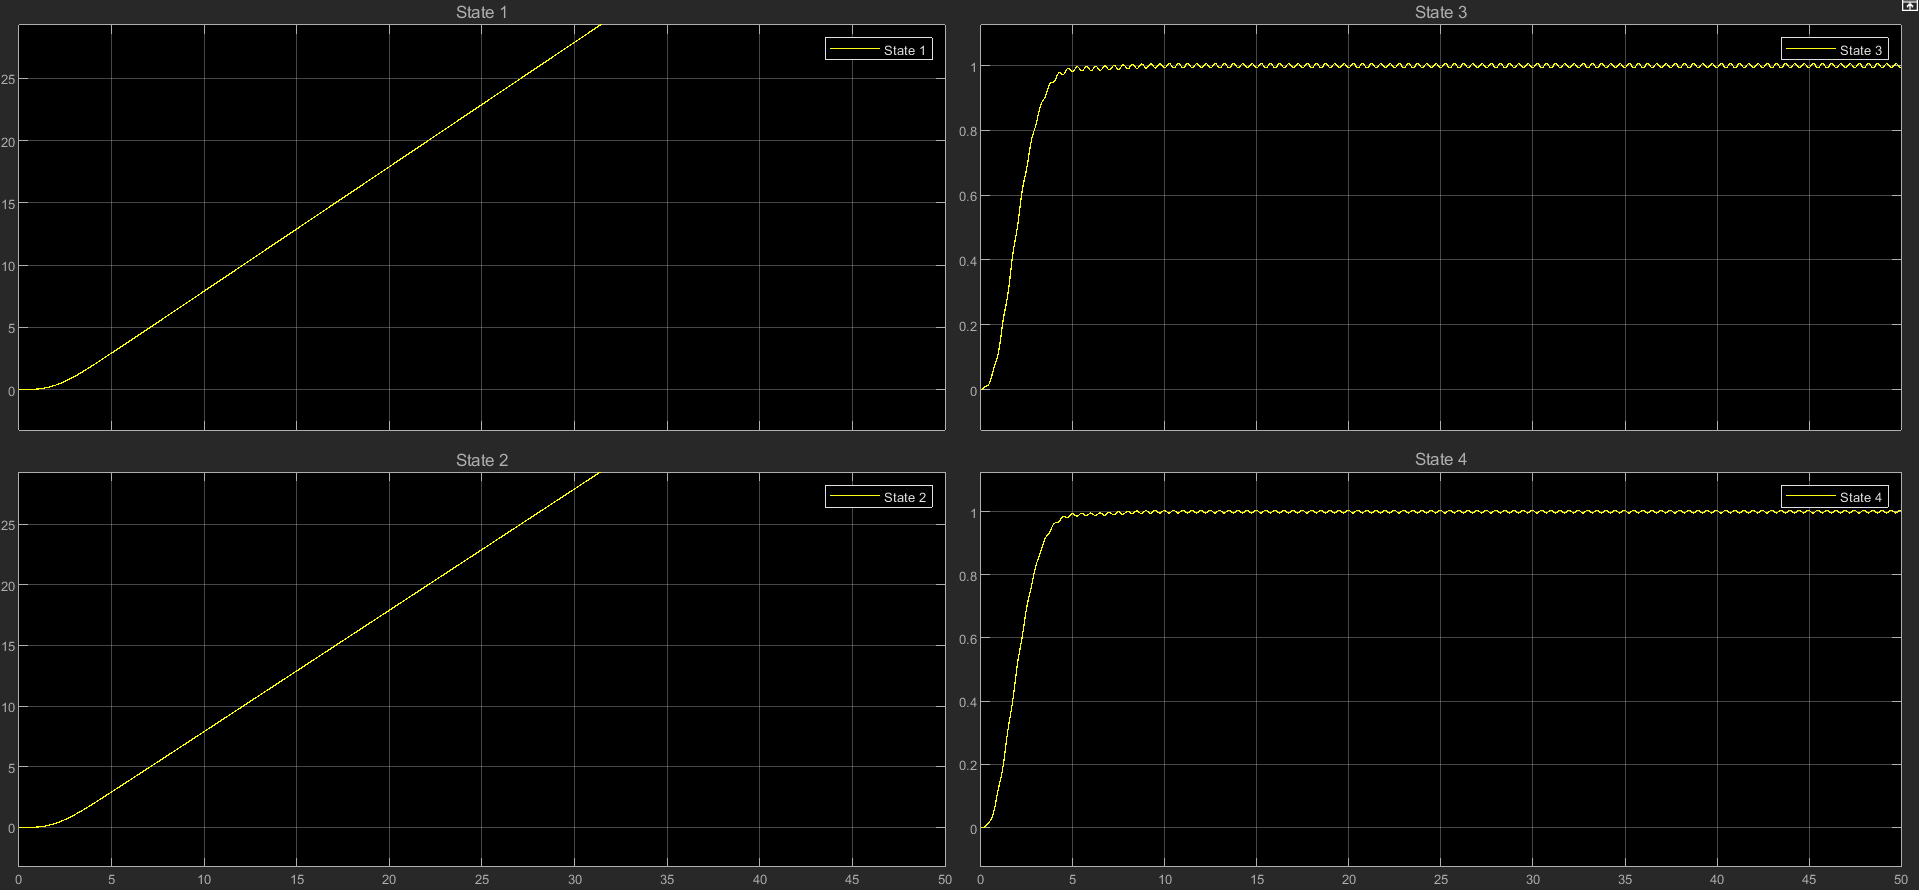
\includegraphics[width=1\linewidth]{../img/Q3_High_disturbance}
	\caption{نمودار خروجی سیستم با اغتشاش}
	\label{fig:q3highdisturbance}
\end{figure}
\begin{figure}[H]
	\centering
	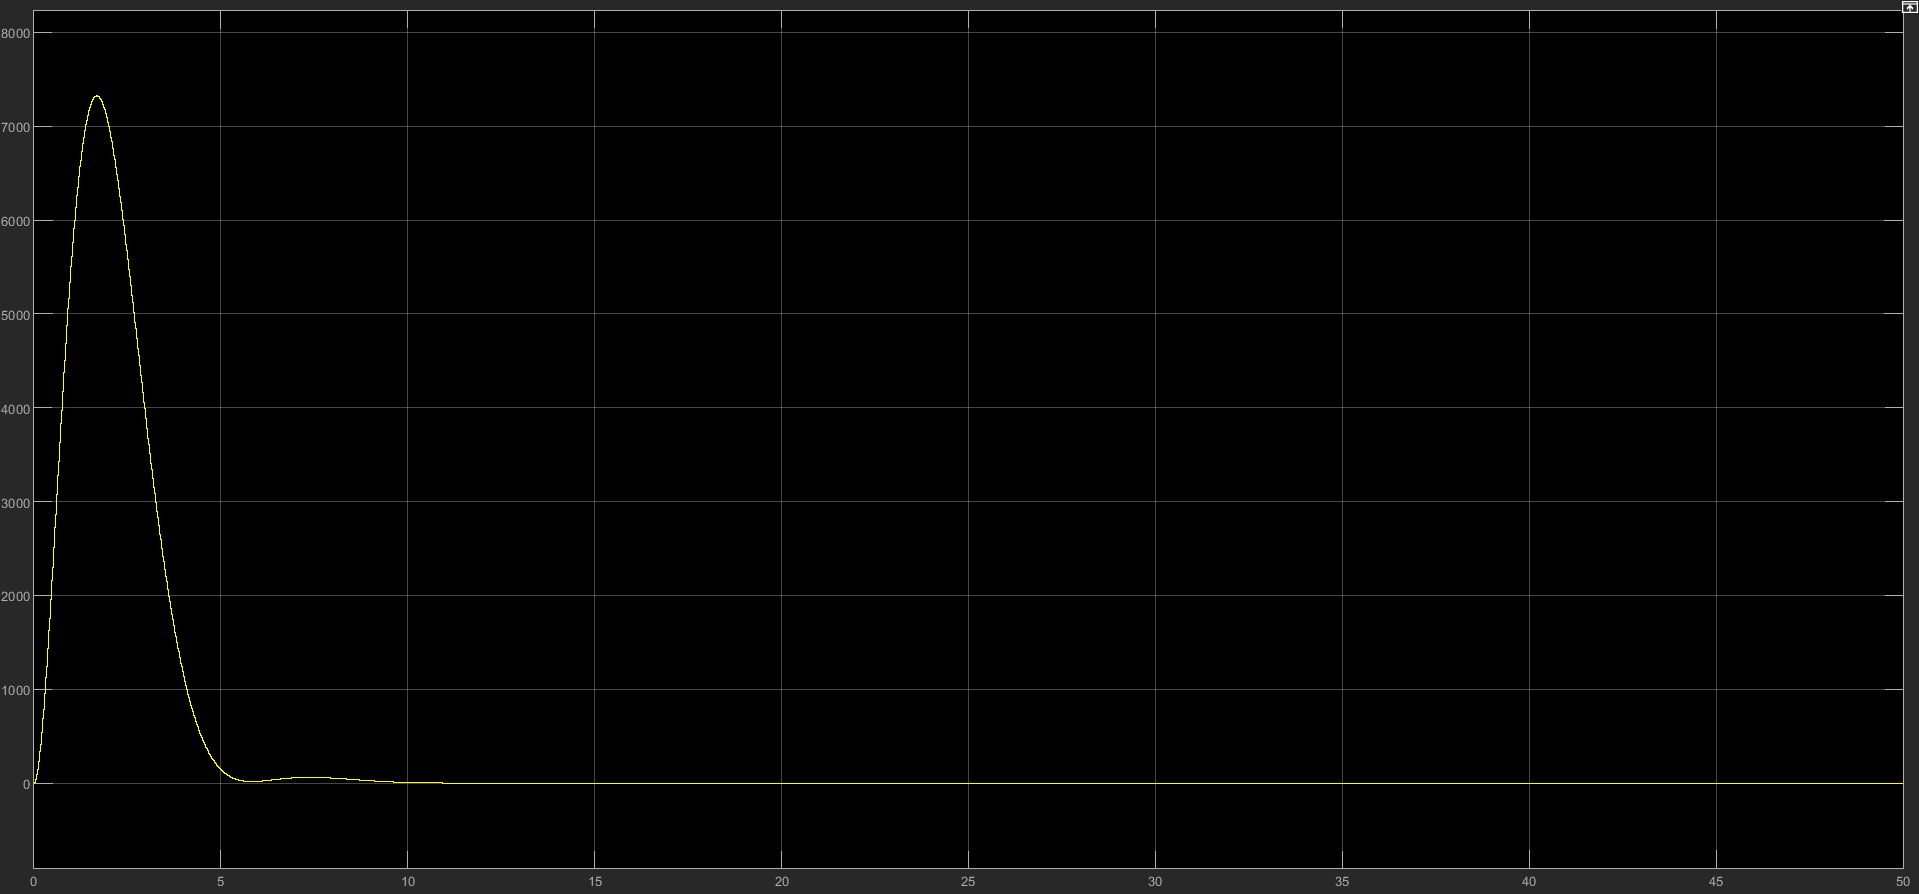
\includegraphics[width=1\linewidth]{../img/Q3_High_disturbance_Ceffort}
	\caption{نمودار تلاش کنترلر}
	\label{fig:q3highdisturbanceceffort}
\end{figure}
در این قسمت، با اضافه کردن یک بلوک کنترلر PID به سیستم، کنترلر $Tube MPC$ را تشکبل داده و نتایج سیستم را مجددا بررسی می کنیم.
ضرایب این کنترلر به دلیل حجم زیاد محاسبات، به وسیله تنظیم کننده متلب قابل تنظیم نبوده و به صورت دستی بر روی ضرایب زیر تنظیم شده است.
\begin{figure}[H]
	\centering
	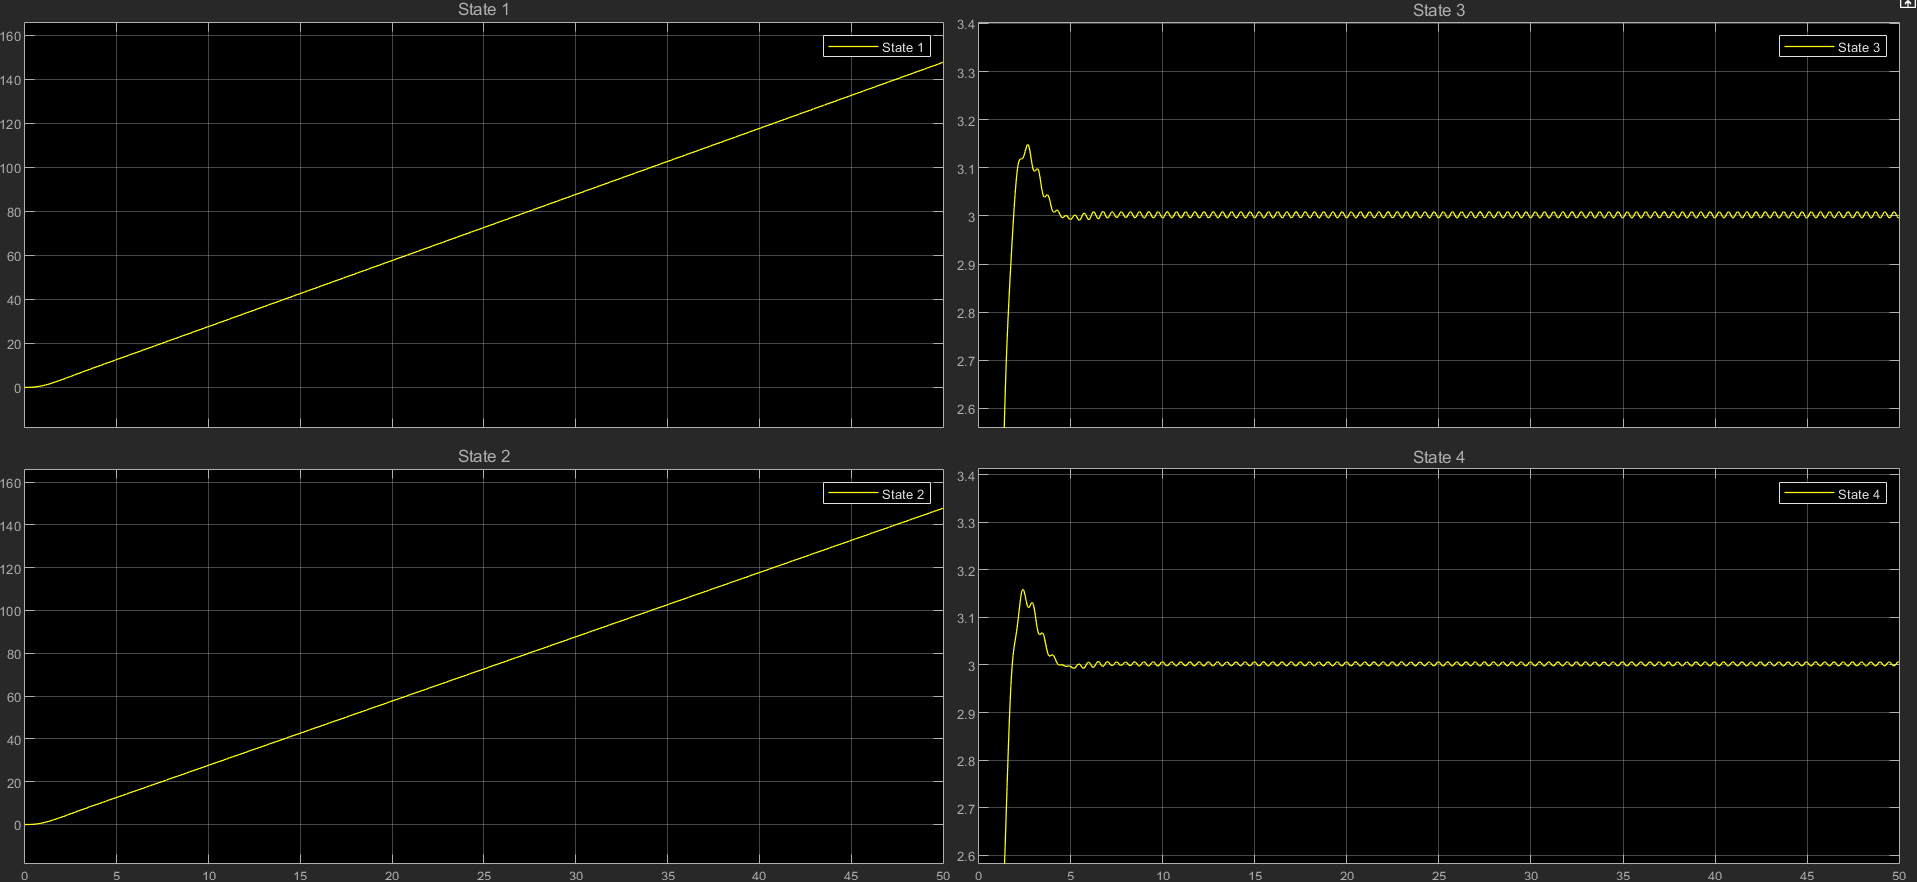
\includegraphics[width=1\linewidth]{../img/Q3_High_disturbance_Tube_Response}
	\caption{نمودار خروجی های حالت سیستم}
	\label{fig:q3highdisturbancetuberesponse}
\end{figure}
\begin{figure}[H]
	\centering
	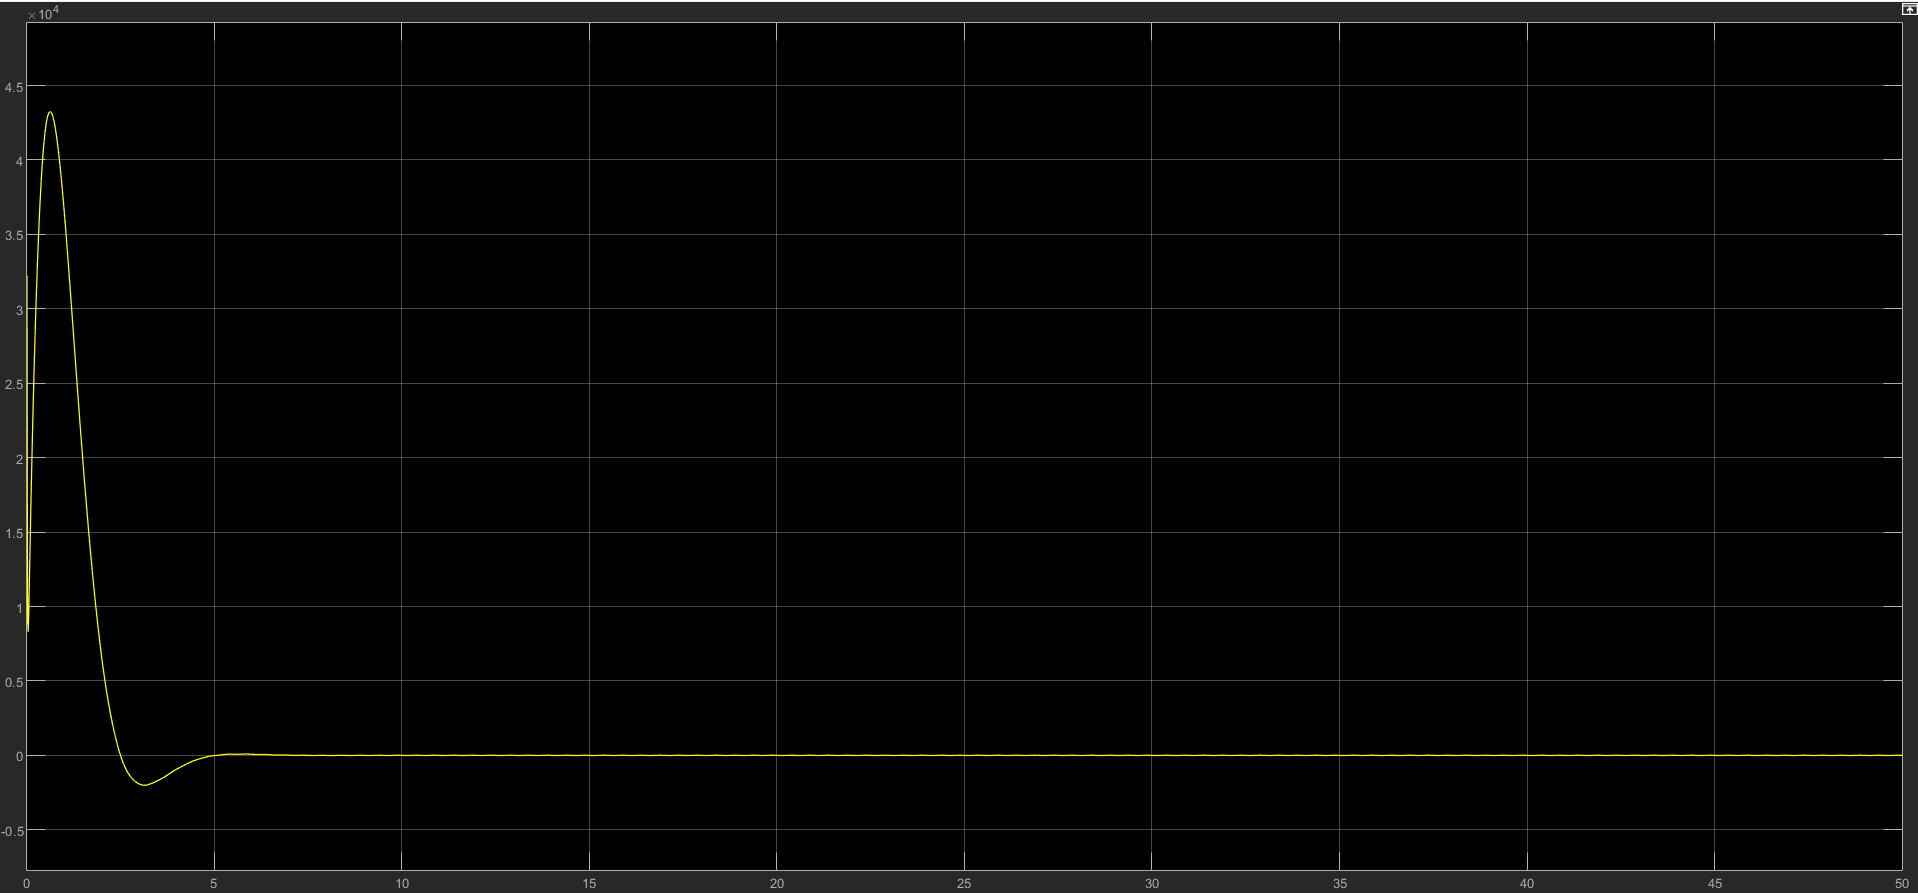
\includegraphics[width=1\linewidth]{../img/Q3_High_disturbance_Tube_Ceffort}
	\caption{نمودار تلاش کنترلر}
	\label{fig:q3highdisturbancetubeceffort}
\end{figure}
\begin{figure}[H]
	\centering
	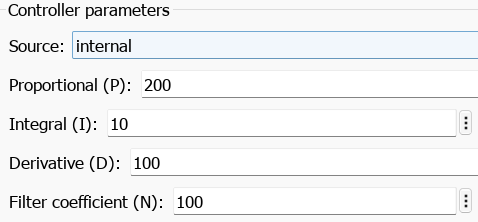
\includegraphics[width=1\linewidth]{../img/Q3_High_disturbance_Tube_PID}
	\caption{ضرایب PID}
	\label{fig:q3highdisturbancetubepid}
\end{figure}
\subsection*{پاسخ بخش چهارم}
در این بخش، با اعمال مقادیری نایقینی مطابق آنچه که در صورت سوال ذکر شده است، به سیستم اعمال می کنیم. برای این کار، به مقادیر ورودی ها، مقادیر سینوسی متغیر با زمان با میزان مشخص شده اضافه می کنیم. سپس، مقادیر خروجی را با استفاده از کنترلر $Tube MPC$ و $Linear MPC$ طراحی شده کنترل می کنیم. 
سیستم کنترلی پیش بین خطی مطابق سیستم زیر مورد استفاده قرار گرفته است.
\begin{figure}[H]
	\centering
	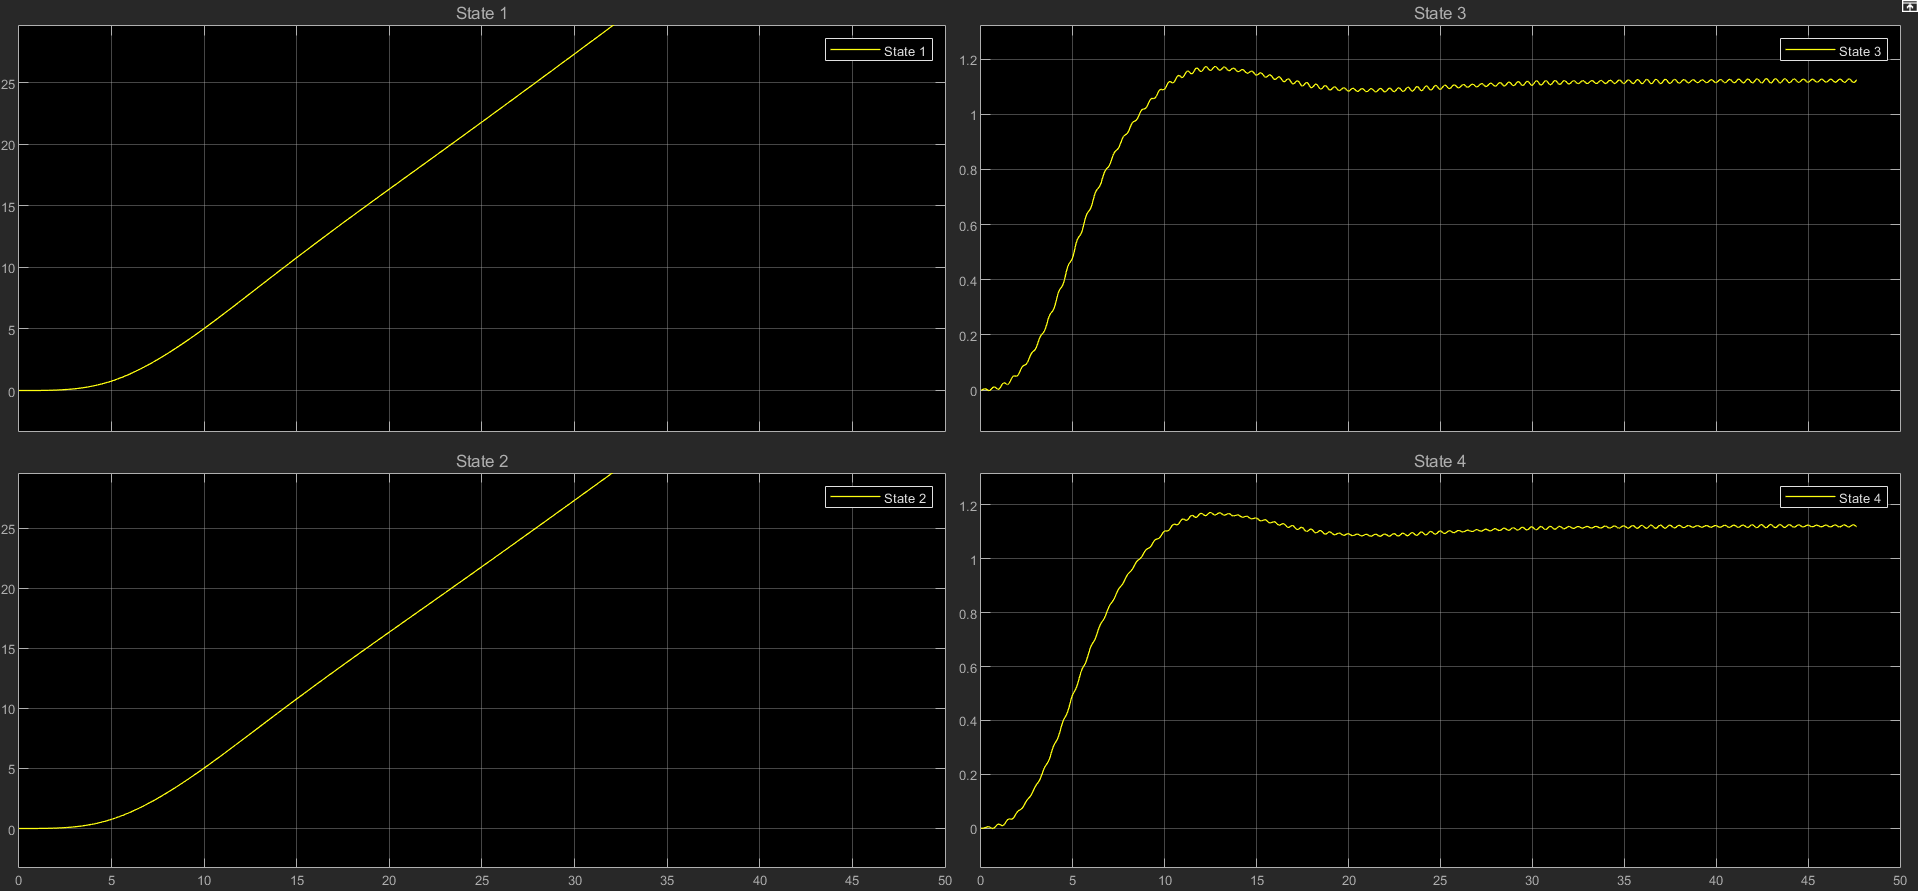
\includegraphics[width=0.7\linewidth]{../img/Q4_Uncertainty_Responce_LinearMPC}
	\caption{نمودار خروجی با وجود نایقینی}
	\label{fig:q4uncertaintyresponcelinearmpc}
\end{figure}
\begin{figure}[H]
	\centering
	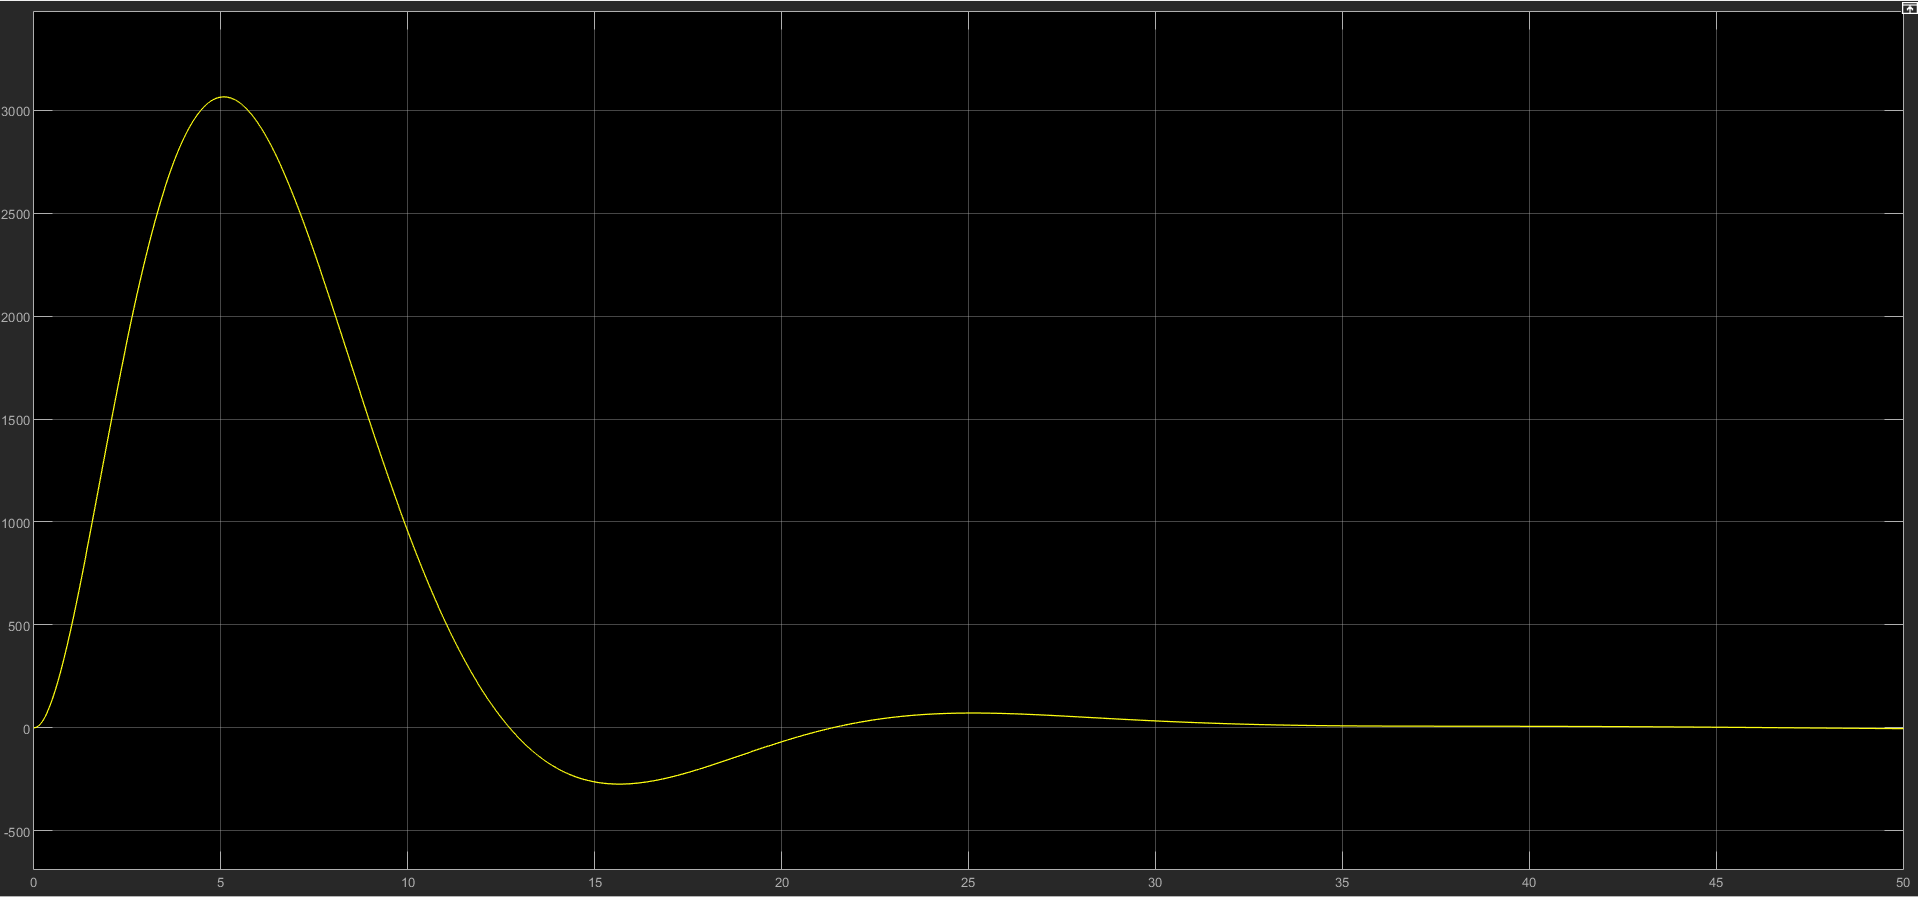
\includegraphics[width=0.7\linewidth]{../img/Q4_Uncertainty_Ceffort_LinearMPC}
	\caption{نمودار تلاش کنترلی با وجود نایقینی}
	\label{fig:q4uncertaintyceffortlinearmpc}
\end{figure}
در ادامه، با تغییر کنترلر به Tube MPC، مجددا سیگنال های کنترلی را بررسی می کنیم.
\begin{figure}[H]
	\centering
	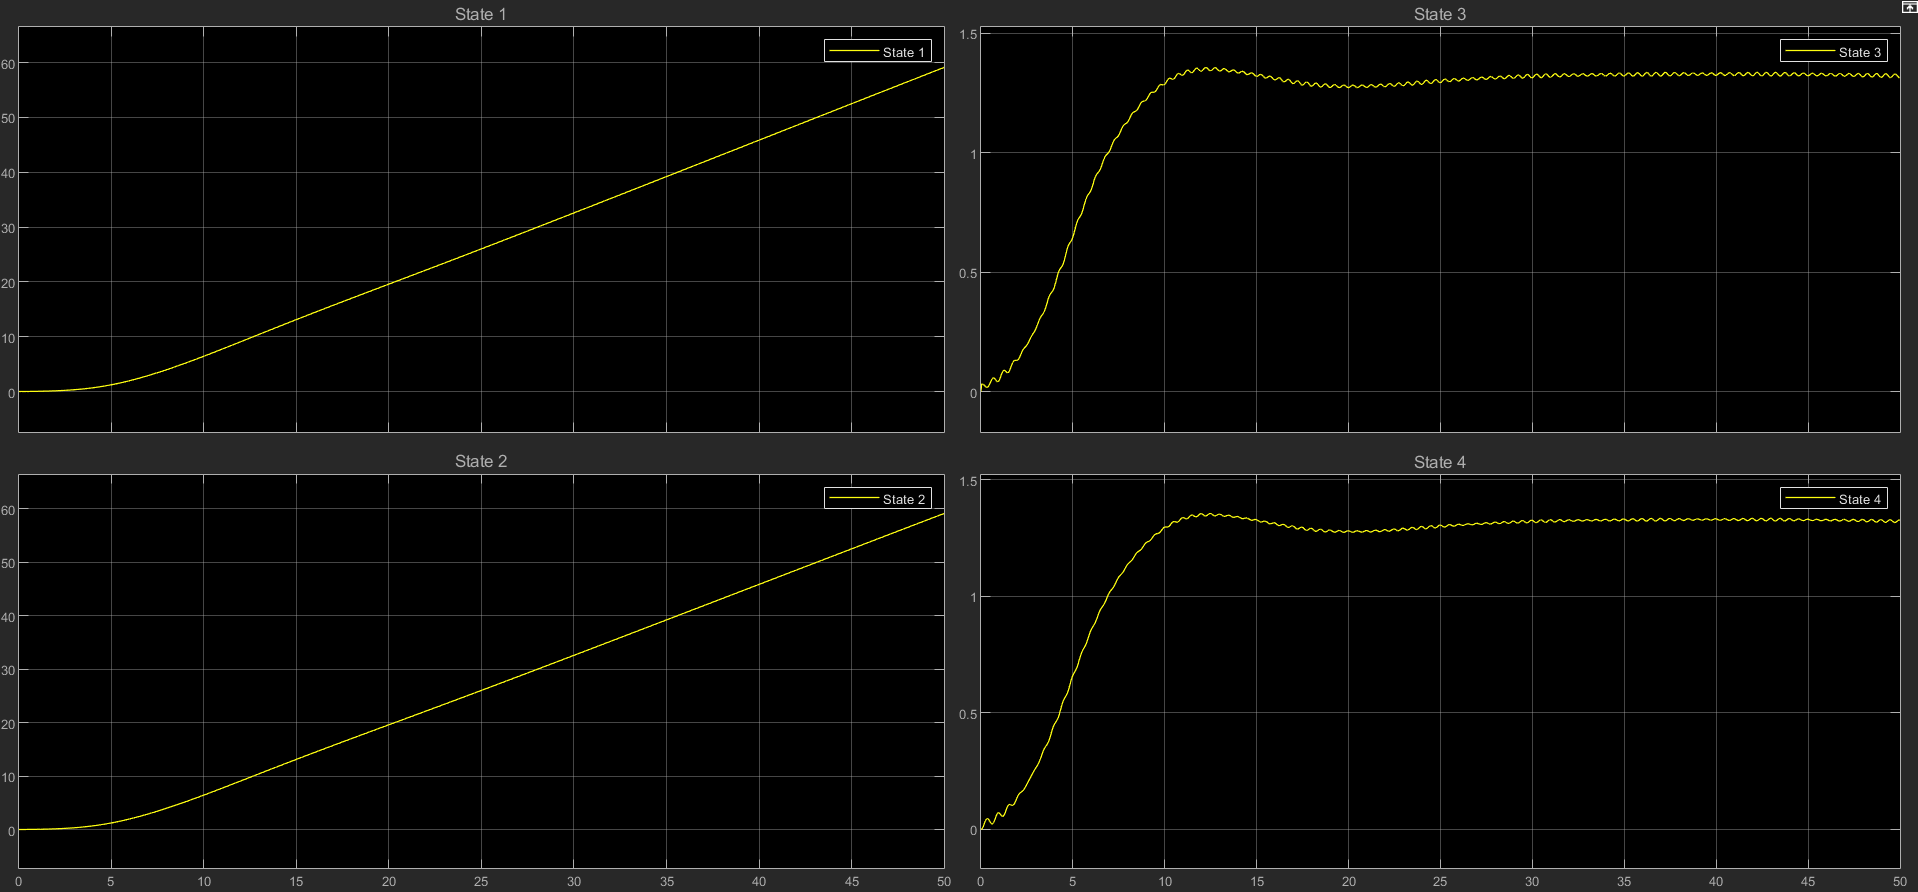
\includegraphics[width=0.7\linewidth]{../img/Q4_Uncertainty_Responce_TubeMPC}
	\caption{نمودار خروجی سیستم با وجود نایقینی}
	\label{fig:q4uncertaintyresponcetubempc}
\end{figure}
\begin{figure}[H]
	\centering
	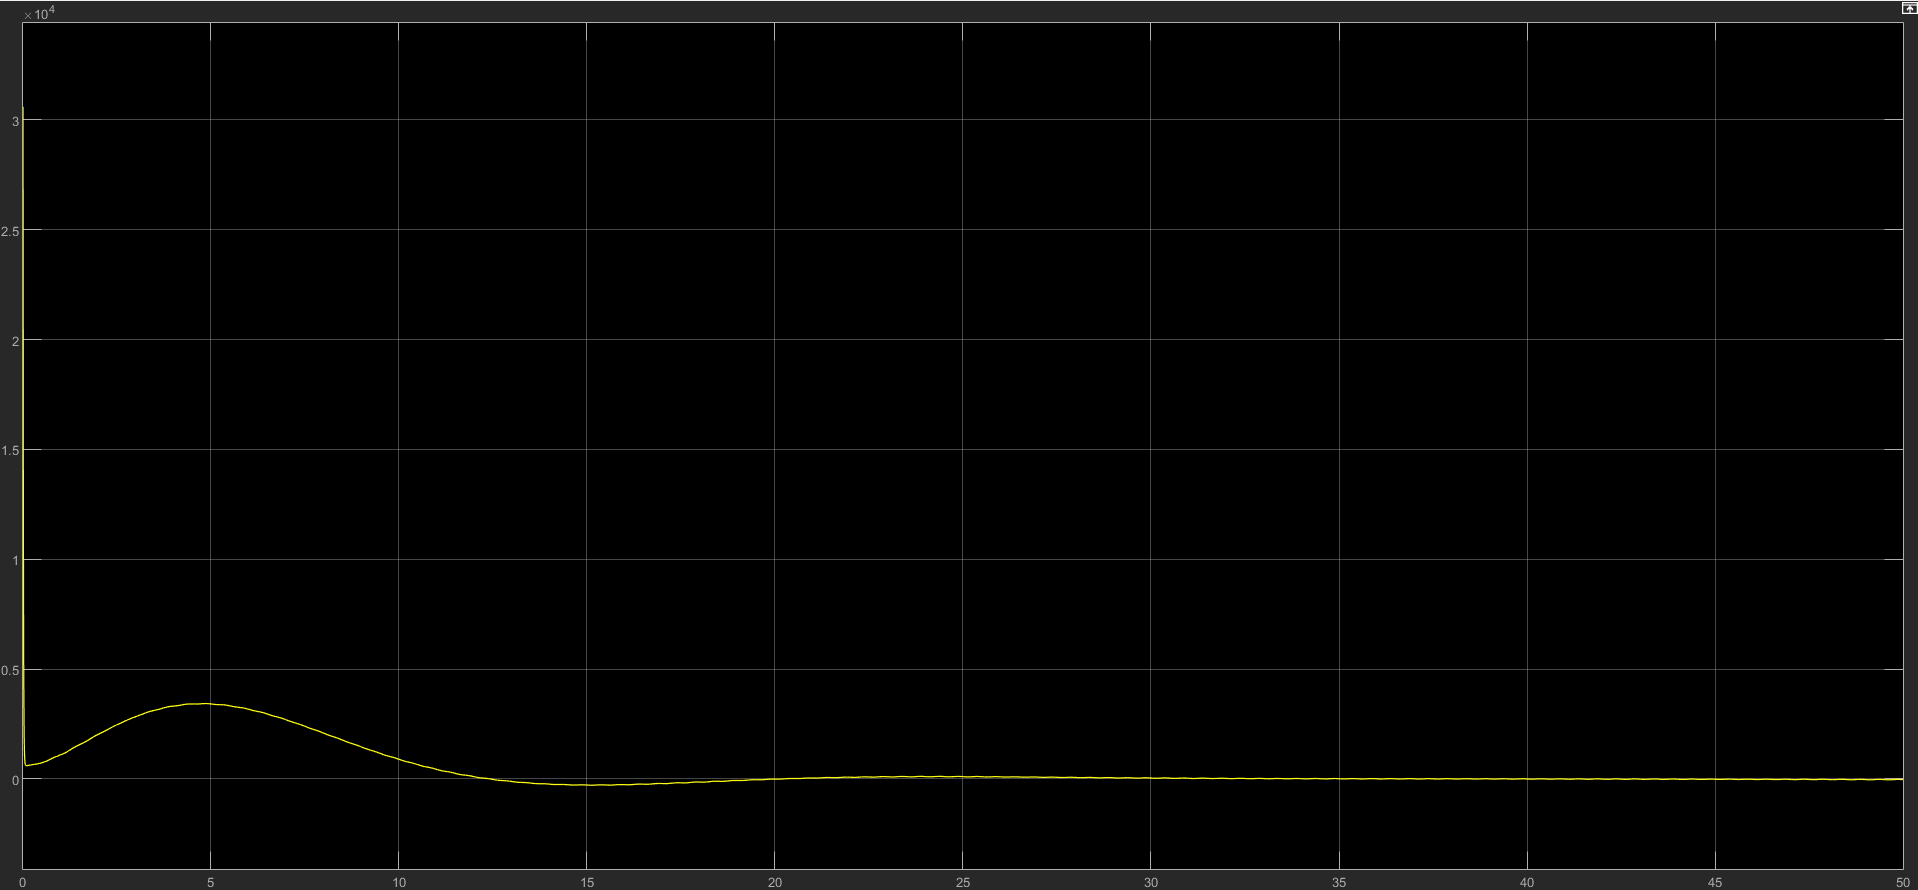
\includegraphics[width=0.7\linewidth]{../img/Q4_Uncertainty_Ceffort_TubeMPC}
	\caption{نمودار خروجی کنترلر بار وجود نایقینی}
	\label{fig:q4uncertaintycefforttubempc}
\end{figure}


